% =============================================================================
%  RVBL-2, ChampionCHIP eXperience Phase 2, Design Submission Report
%
%  Build:   pdflatex RVBL2_ChampionCHIP_Report.tex   (run twice for references)
%
%  This file compiles with NO external images present. Every \includegraphics
%  is wrapped in \IfFileExists and degrades to a visible placeholder box that
%  tells you exactly how to produce the missing image.
%
%  TO FINISH THIS REPORT:
%    1. Set \videourl and \repourl below (marked TODO). The video URL is
%       REQUIRED by Submission Guide 7 and 9.
%    2. Drop the screenshots listed in the placeholder boxes into report/figures/
%       using EXACTLY the filenames the boxes name.
%    3. Add raster screenshots at <= 150 dpi. The 17 ChipInventor block icons
%       already contribute ~3 MB; the Guide's limit is 10 MB.
% =============================================================================
\documentclass[11pt,a4paper]{article}

\usepackage[T1]{fontenc}
\usepackage[utf8]{inputenc}
% Latin Modern: scalable Type 1 outlines. Required for microtype's font
% expansion -- the default EC fonts are bitmaps and cannot be expanded.
\usepackage{lmodern}
\usepackage[a4paper,top=20mm,bottom=18mm,left=19mm,right=19mm,headheight=22pt,
            footskip=12mm]{geometry}
\usepackage{graphicx}
\usepackage{booktabs}
\usepackage{tabularx}
\usepackage{longtable}
\usepackage[table]{xcolor}
\usepackage{listings}
\usepackage{tikz}
\usepackage{caption}
\usepackage{subcaption}
\usepackage{enumitem}
\usepackage{fancyhdr}
\usepackage{amsmath}
\usepackage{amssymb}
\usepackage{multirow}
\usepackage{float}
\usepackage{microtype}

\usetikzlibrary{arrows.meta,positioning,calc,fit,shapes.geometric,backgrounds}

% ------------------------------------------------------------------ palette --
% Defined BEFORE hyperref, because hyperref's link colours reference them.
\definecolor{rvbl}{HTML}{0E5C63}        % accent -- headings, rules, callouts
\definecolor{rvbldark}{HTML}{08383D}    % links, subheadings
\definecolor{rvbltint}{HTML}{E4EFF0}    % table header fill
\definecolor{rvblsoft}{HTML}{F4F9F9}    % box fill
\definecolor{rvblrule}{HTML}{5C9298}    % table rules
\definecolor{okgreen}{HTML}{1B6B3A}
\definecolor{warnamber}{HTML}{8A5A00}
\definecolor{codebg}{HTML}{F6F6F3}

\arrayrulecolor{rvblrule}

\usepackage{hyperref}
\hypersetup{
  colorlinks=true, linkcolor=rvbldark, citecolor=rvbldark, urlcolor=rvbldark,
  pdftitle={RVBL-2 Multicycle RISC-V Processor: ChampionCHIP eXperience Phase 2
            Design Submission Report},
  pdfauthor={Equipe 13},
  pdfsubject={RV32I + Zmmul + Xicrc multicycle RISC-V core: architecture, ISA coverage,
              datapath, modules and testbenches, OpenLane physical implementation, and
              official validation-firmware demonstration},
  pdfkeywords={RISC-V, RV32I, Zmmul, Xicrc, multicycle, ChipInventor, OpenLane, Sky130,
               GDSII, ChampionCHIP}
}

% \needlines{n}: start a new page unless n lines still fit. Used before a
% heading so a section never appears as the last item on a page.
\newcommand{\needlines}[1]{%
  \par
  \ifdim\pagegoal=\maxdimen\else
    \ifdim\dimexpr\pagegoal-\pagetotal\relax<\dimexpr#1\baselineskip\relax
      \newpage
    \fi
  \fi}

% ------------------------------------------------------- headings (no titlesec)
\makeatletter
\renewcommand\section{\@startsection{section}{1}{\z@}%
  {-2.6ex \@plus -1ex \@minus -.2ex}{1.2ex \@plus.2ex}%
  {\color{rvbl}\normalfont\large\bfseries}}
\renewcommand\subsection{\@startsection{subsection}{2}{\z@}%
  {-2.1ex\@plus -1ex \@minus -.2ex}{0.7ex \@plus .2ex}%
  {\color{rvbldark}\normalfont\normalsize\bfseries}}
\renewcommand\subsubsection{\@startsection{subsubsection}{3}{\z@}%
  {-1.6ex\@plus -1ex \@minus -.2ex}{-0.6em}%
  {\color{rvbldark}\normalfont\normalsize\bfseries}}
\makeatother

\captionsetup{font=small,labelfont={bf,color=rvbl},skip=4pt,
              justification=justified,singlelinecheck=false}
\captionsetup[sub]{font=footnotesize,labelfont={bf,color=rvbl}}

\pagestyle{fancy}
\fancyhf{}
\renewcommand{\headrulewidth}{0.4pt}
\renewcommand{\headrule}{\hbox to\headwidth{\color{rvblrule}\leaders\hrule height
  \headrulewidth\hfill}}
\fancyhead[L]{\footnotesize\color{rvbl}RVBL-2 Multicycle RISC-V Processor}
\fancyhead[R]{\footnotesize\color{rvbl}Equipe 13 \textbullet{} ChampionCHIP eXperience, Phase 2}
\fancyfoot[C]{\footnotesize\thepage}

\setlist[itemize]{leftmargin=1.3em,itemsep=1pt,topsep=2pt,parsep=0pt}
\setlist[enumerate]{leftmargin=1.5em,itemsep=1pt,topsep=2pt,parsep=0pt}
\setlength{\parskip}{3pt}
\setlength{\parindent}{0pt}
% Absorb the last few marginal overfull lines caused by long \texttt identifiers.
\setlength{\emergencystretch}{2.5em}
% Float placement: allow pages to be filled rather than leaving large gaps.
\renewcommand{\topfraction}{0.85}
\renewcommand{\bottomfraction}{0.60}
\renewcommand{\textfraction}{0.12}
\renewcommand{\floatpagefraction}{0.75}
% On a float-only page put all the slack at the bottom. The default spreads it
% between the floats, which looks like a hole in the middle of the page.
\makeatletter
\setlength{\@fptop}{0pt}
\setlength{\@fpsep}{14pt plus 0fil}
\setlength{\@fpbot}{0pt plus 1fil}
\makeatother
\setcounter{topnumber}{3}
\setcounter{bottomnumber}{2}
\setcounter{totalnumber}{5}
\renewcommand{\arraystretch}{1.12}

% ------------------------------------------------------------------- listings --
\lstdefinestyle{loglisting}{
  basicstyle=\ttfamily\scriptsize,
  backgroundcolor=\color{codebg},
  frame=leftline, framerule=1.6pt, rulecolor=\color{rvblrule},
  framexleftmargin=5pt, xleftmargin=7pt, xrightmargin=2pt,
  breaklines=true, columns=fullflexible, keepspaces=true,
  showstringspaces=false, aboveskip=5pt, belowskip=3pt
}
\lstset{style=loglisting}

% --------------------------------------------------------------------- macros --
% ******************** THE TWO THINGS YOU MUST EDIT ***************************
% 1. The demonstration video. Submission Guide sections 7 and 9 both require
%    this URL in the report. Printed on the title page and again in section 6.
\newcommand{\videourl}{https://youtu.be/TODO-REPLACE-WITH-YOUR-VIDEO-ID}
%
% 2. The public repository. Printed beside the video URL, and used to build a
%    direct link to the full-resolution architecture diagram under Figure 5.
%    No trailing slash.
\newcommand{\repourl}{https://github.com/TODO-USER/TODO-REPO}
% *****************************************************************************

% Built from \repourl, so setting the repository URL fixes this link too.
\newcommand{\diagramurl}{\repourl/blob/main/report/figures/soc-architecture.png}

% \fullresbar{<name>} prints the "view this diagram full size" control under
% a dense figure. An earlier version embedded the image as a PDF file
% attachment; that was dropped because browser PDF viewers ignore attachments
% outright and desktop readers rendered it as an invisible hotspot. A plain
% https link works everywhere and survives printing.
\newcommand{\fullresbar}[1]{%
  \par\vspace{2pt}%
  \begin{center}\scriptsize
    \href{\diagramurl}{\color{rvbl}\bfseries View this diagram full size}%
    \ {\color{rvblrule}(opens the image in the project repository)}\par\vspace{1pt}
    Or zoom to 300\,\% in any reader: stored here at about 580\,dpi\,$\cdot$\,
    the same image is in the submission as \texttt{#1}%
  \end{center}\par\vspace{2pt}}

% Single knob for how tall any supplied screenshot may be. Every figure is capped
% at this, so the document stays at 20 pages whatever aspect ratios you drop in.
% Verified at 20 pages both with no images at all and with all nine present.
% If you add images and the PDF spills to 21 pages, reduce this one value.
\newcommand{\figmaxh}{0.26\textheight}

\newcommand{\needsimage}[2]{%
  \begin{center}%
  \setlength{\fboxsep}{8pt}%
  \fbox{\parbox{0.86\linewidth}{\centering
    \vspace{0.3em}\par
    \textbf{[IMAGE PLACEHOLDER]}\par\vspace{0.3em}
    % \detokenize so underscores in the filename do not start math mode
    \texttt{\detokenize{#1}}\par\vspace{0.3em}
    {\footnotesize #2}\par\vspace{0.3em}}}%
  \end{center}}

% #1 path  #2 width  #3 how-to-produce note  #4 caption  #5 label
% The height cap matters: it keeps the page count stable when the real
% screenshots replace the placeholders, whatever aspect ratio they have.
\newcommand{\figorbox}[5]{%
  \begin{figure}[htbp]\centering
  \IfFileExists{#1}%
    {\includegraphics[width=#2,height=\figmaxh,keepaspectratio]{#1}}%
    {\needsimage{#1}{#3}}%
  \caption{#4}\label{#5}\end{figure}}

% Zero-width break opportunities, so long \texttt identifiers and paths can wrap
% inside narrow table columns instead of overflowing into the margin.
\newcommand{\pb}{\discretionary{}{}{}}       % break here, print nothing
\newcommand{\ub}{\_\discretionary{}{}{}}     % underscore, then allow a break

\newcommand{\hdr}[1]{\textbf{#1}}
% Default overhang on purpose. colortbl paints a row colour one \tabcolsep
% beyond each cell, and the optional [l][r] arguments apply to EVERY cell,
% not just the outer two -- so zeroing them breaks the band into one
% segment per column. The band is kept whole here, and the tables instead
% do NOT trim their outer @{}, so the rules span the same extent the band
% already covers and the two line up.
\newcommand{\hrow}{\rowcolor{rvbltint}}
\newcommand{\ok}{\textcolor{okgreen}{\textbf{PASS}}}
\newcommand{\zero}{\textcolor{okgreen}{\textbf{0}}}

% callout box -- rules rather than a spanning \colorbox, so it is robust
% A callout must be able to split across a page boundary. An earlier version
% wrapped the body in a minipage, which cannot break: when the page was full
% the box silently ran off the bottom edge and over the page number. This
% version uses a plain list, so TeX breaks it like ordinary text.
% One unbreakable unit, so a callout never starts a page in mid-sentence.
% \penalty-150 in front gives TeX a legal and attractive place to break, which
% is what lets the whole box move to the next page instead of overrunning the
% bottom margin. Without that penalty a preceding heading or float can leave
% no breakpoint at all.
\newenvironment{callout}[1]{%
  \par\penalty-150\vspace{6pt}%
  \begin{center}\begin{minipage}{0.965\linewidth}%
  \textcolor{rvbl}{\rule{\linewidth}{0.9pt}}\par\vspace{1pt}%
  {\color{rvbl}\bfseries #1}\par\vspace{2pt}\small\ignorespaces}%
 {\par\vspace{3pt}\textcolor{rvbl}{\rule{\linewidth}{0.9pt}}%
  \end{minipage}\end{center}\vspace{4pt}\par}

\begin{document}

% =============================================================================
% PAGE 1 -- TITLE + AT-A-GLANCE
% =============================================================================
\thispagestyle{fancy}

\begin{center}
{\color{rvbl}\rule{\linewidth}{2pt}}\\[10pt]
{\Huge\bfseries\color{rvbl} RVBL-2}\\[4pt]
{\LARGE\bfseries A Multicycle RISC-V Processor}\\[8pt]
{\large RV32I \,+\, Zmmul \,+\, Xicrc \textbullet{} 47 instructions \textbullet{} SkyWater Sky130A}\\[10pt]
{\color{rvbl}\rule{\linewidth}{2pt}}\\[8pt]
{\large\textbf{ChampionCHIP eXperience: Phase 2 Design Submission Report}}\\[7pt]
{\large\color{rvbl}\textbf{Equipe 13}}\\[6pt]
{\normalsize Implemented on the ChipInventor platform \textbullet{} Taped out through
OpenLane to signed-off GDSII}\\[10pt]
\end{center}

\vspace{2pt}
\begin{center}
\small
\begin{tabularx}{\linewidth}{lX@{\hspace{1.4em}}lX}
\toprule
\hdr{ISA} & RV32I (37) + Zmmul (4) + Xicrc (3) = \textbf{47/47, 100\,\%}
  & \hdr{Die} & \textbf{0.404\,mm$^2$} (630.15\,$\times$\,640.87\,\textmu m) \\
\hdr{Microarchitecture} & 6-state multicycle FSM, 3--5 cycles/instruction
  & \hdr{Density} & \textbf{52.28\,\%} final core utilisation \\
\hdr{Validation firmware} & \textbf{\textcolor{okgreen}{PASS}: \texttt{x4 = 0x00000000}},
  9/9 stages, 991 cycles
  & \hdr{Cells / flops} & \textbf{17{,}708} / \textbf{1{,}393} \\
\hdr{Verification} & 7{,}384 checks (15 TBs) + 15{,}281 checks (platform suite)
  & \hdr{Timing} & setup \textbf{+2.25\,ns} slow corner; hold +0.11\,ns \\
\hdr{Equivalence} & 410{,}400 lockstep comparisons, 0 mismatches
  & \hdr{Signoff} & \zero{} DRC \textbullet{} \zero{} routing viol.
    \textbullet{} LVS match uniquely \\
\hdr{Technology} & sky130A, \texttt{sky130\_fd\_sc\_hd}, no macros
  & \hdr{Clock} & 33\,ns constraint; closes at $\approx$32.5\,MHz \\
\bottomrule
\end{tabularx}
\end{center}

\vspace{2pt}
\begin{center}
\setlength{\fboxsep}{8pt}%
\fcolorbox{rvbl}{rvblsoft}{\begin{minipage}{0.94\linewidth}\centering
{\color{rvbl}\bfseries\large Project demonstration video (Submission Guide \S7 / \S9)}\\[4pt]
\large\url{\videourl}\\[6pt]
{\color{rvbl}\bfseries\large Source, testbenches and full-resolution figures}\\[4pt]
\large\url{\repourl}
\end{minipage}}
\end{center}

\vspace{10pt}
\figorbox{figures/gds_layout.png}{0.46\linewidth}
  {Decorative title image.}
  {The finished RVBL-2 chip. The die is 630.15\,$\times$\,640.87\,\textmu m and holds 17{,}708 standard cells in 0.404\,mm$^2$. The pink bands at the top and bottom are power and filler rows. The blue area is the routed logic.}
  {fig:die}

\vfill
{\footnotesize\color{rvbl}\rule{\linewidth}{0.6pt}}\\[2pt]
{\footnotesize Every number in this report is measured, not estimated. Each one comes from a
tool report or a test run in the submission, and this report says which. The section
numbers follow the Submission Guide's own topics 1 to 6.}

\newpage

% =============================================================================
% PAGE 2 -- COMPLIANCE MAP + EVIDENCE CHAIN
% =============================================================================
\section*{\color{rvbl}Requirements compliance: where each requirement is answered}
\addcontentsline{toc}{section}{Requirements compliance}
\label{sec:compliance}

\vspace{-2pt}
{\small
\begin{tabularx}{\linewidth}{c>{\raggedright\arraybackslash}p{3.5cm}Xc}
\toprule
\hrow \hdr{Guide \S} & \hdr{Requirement} & \hdr{How it is answered} & \hdr{Page} \\
\midrule
1 & Project Overview & Goal, multicycle architecture, 20 modules, general operation,
    RISC-V functionality implemented (\S\ref{sec:overview}) & \pageref{sec:overview} \\
2 & Supported Instructions & Coverage grouped by ISA category, expected-vs-implemented
    summary, per-category lists, full 47-row encoding table (\S\ref{sec:isa}) &
    \pageref{sec:isa} \\
3 & Datapath & Complete datapath with control unit, data flow between all modules,
    FSM, per-class cycle counts (\S\ref{sec:datapath}) & \pageref{sec:datapath} \\
4 & Modules and Testbenches & All 17 ChipInventor blocks, their ports, their
    testbenches, and the ChipInventor block diagrams (\S\ref{sec:modules}) &
    \pageref{sec:modules} \\
5 & OpenLane Results & Total area, density, signoff results and the final GDSII image
    (\S\ref{sec:openlane}) & \pageref{sec:openlane} \\
6 & Firmware Demo & All 9 validation stages, waveforms, and verbatim testbench log
    output showing the run reached the end without errors (\S\ref{sec:firmware}) &
    \pageref{sec:firmware} \\
7 & Video Demo & URL on the title page and in \S\ref{sec:deliverables} &
    \pageref{sec:compliance} \\
8 & Report Format & PDF, within 20 pages and 10\,MB, covering topics 1--6 & n/a \\
9 & Expected Files & Deliverables map, \S\ref{sec:deliverables} &
    \pageref{sec:deliverables} \\
\bottomrule
\end{tabularx}}

\vspace{4pt}
\subsection*{\color{rvbldark}The central claim: the chip that was taped out is the design
that was verified}

Most submissions can show that their RTL passes a testbench and, separately, that
\emph{something} went through OpenLane. This project can show that they are the same
design, by mechanical check rather than assertion. Figure~\ref{fig:chain} is the whole
argument; every count in it was produced by a script in the repository and reproduced while
this report was being written.

\begin{figure}[htbp]
\centering
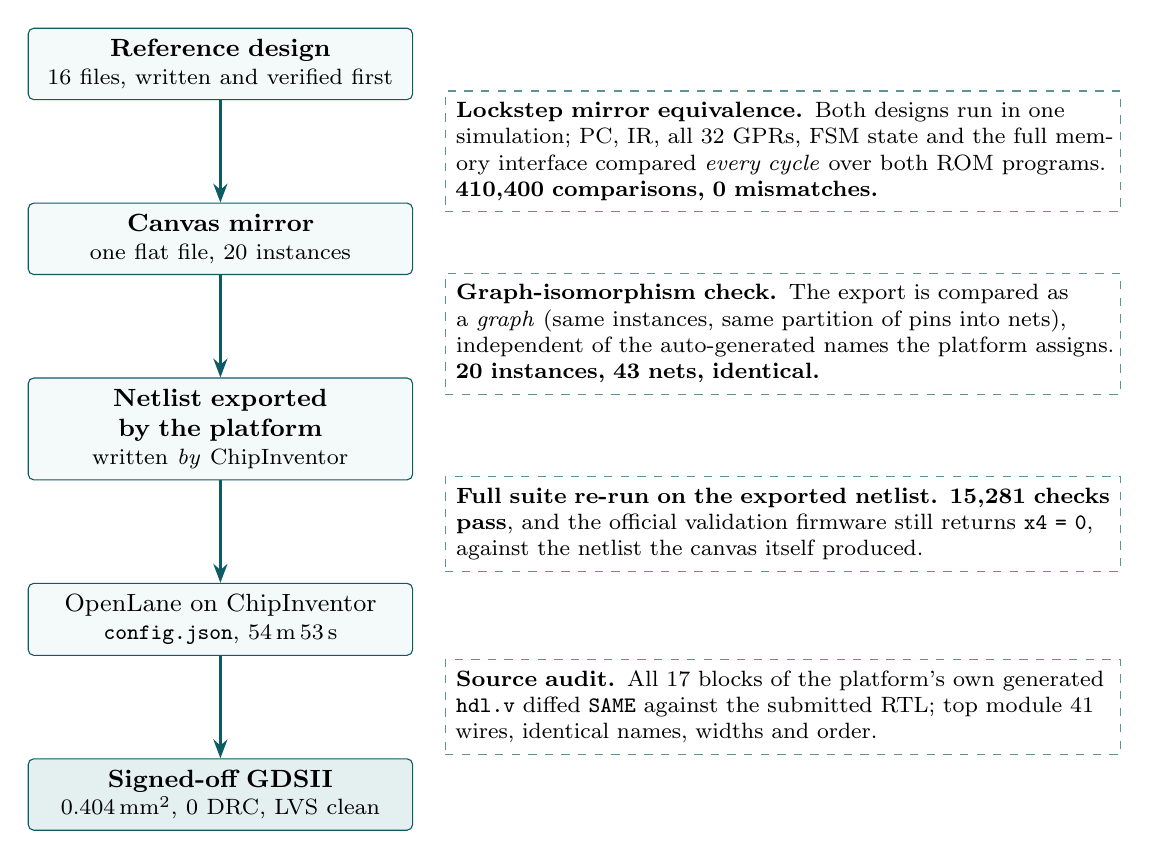
\begin{tikzpicture}[
  font=\small,
  node distance=0pt,
  art/.style={draw=rvbl,fill=rvblsoft,rounded corners=2pt,text width=4.6cm,align=center,
              inner sep=4pt,minimum height=8mm},
  chk/.style={draw=rvblrule,dashed,fill=white,text width=8.3cm,align=left,inner sep=4pt,
              font=\footnotesize},
  ar/.style={-{Stealth[length=2.4mm]},rvbl,thick}
]
\node[art] (rtl) at (0,0) {\textbf{Reference design}\\[-1pt]{\footnotesize 16 files,
  written and verified first}};
\node[art,below=13mm of rtl] (ci) {\textbf{Canvas mirror}\\[-1pt]
  {\footnotesize one flat file, 20 instances}};
\node[art,below=13mm of ci] (top) {\textbf{Netlist exported by the platform}\\[-1pt]
  {\footnotesize written \emph{by} ChipInventor}};
\node[art,below=13mm of top] (ol) {OpenLane on ChipInventor\\[-1pt]
  {\footnotesize \texttt{config.json}, 54\,m\,53\,s}};
\node[art,below=13mm of ol,fill=rvbltint] (gds) {\textbf{Signed-off GDSII}\\[-1pt]
  {\footnotesize 0.404\,mm$^2$, 0 DRC, LVS clean}};

\draw[ar] (rtl) -- (ci);
\draw[ar] (ci) -- (top);
\draw[ar] (top) -- (ol);
\draw[ar] (ol) -- (gds);

\node[chk,anchor=west] at ($(rtl.east)!0.5!(ci.east)+(4mm,0)$)
  {\textbf{Lockstep mirror equivalence.} Both designs run in one simulation; PC, IR, all
   32 GPRs, FSM state and the full memory interface compared \emph{every cycle} over both
   ROM programs. \textbf{410{,}400 comparisons, 0 mismatches.}};
\node[chk,anchor=west] at ($(ci.east)!0.5!(top.east)+(4mm,0)$)
  {\textbf{Graph-isomorphism check.} The export is compared as a \emph{graph} (same
   instances, same partition of pins into nets), independent of the auto-generated names
   the platform assigns. \textbf{20 instances, 43 nets, identical.}};
\node[chk,anchor=west] at ($(top.east)!0.5!(ol.east)+(4mm,0)$)
  {\textbf{Full suite re-run on the exported netlist.}
   \textbf{15{,}281 checks pass}, and the official validation firmware still returns
   \texttt{x4 = 0}, against the netlist the canvas itself produced.};
\node[chk,anchor=west] at ($(ol.east)!0.5!(gds.east)+(4mm,0)$)
  {\textbf{Source audit.} All 17 blocks of the platform's own generated \texttt{hdl.v}
   diffed \texttt{SAME} against the submitted RTL; top module 41 wires, identical names,
   widths and order.};
\end{tikzpicture}
\caption{Unbroken evidence chain from reference RTL to signed-off GDSII. Each arrow is a
mechanical check, not a claim: a swapped wire fails at the graph check rather than
surfacing later as a puzzling simulation result. Every check in the chain is
automated and is re-run before each submission.}
\label{fig:chain}
\end{figure}


% =============================================================================
% 1 PROJECT OVERVIEW
% =============================================================================
\section{Project Overview}
\label{sec:overview}

\textbf{In one paragraph.} RVBL-2 is a 32-bit RISC-V processor core. We built it to the
ChipInventor RVBL-2 Block Guide. It executes the complete RV32I base instruction set, the
standard Zmmul multiply extension, and a custom CRC-16 extension called Xicrc. That is 47
instructions.

The core is \emph{multicycle}. Each instruction takes three to five clock cycles, and the
hardware is used again in each cycle. One arithmetic-logic unit (ALU), one memory port and
one register write port therefore serve all instructions. Nothing is duplicated. The Block
Guide requires this arrangement (\S2.1) because it saves area. It also makes the design
easy to verify: instructions never overlap, so no hazard can occur. There is no forwarding
logic, no stall logic and no flush logic to get wrong.

We entered the core on the ChipInventor canvas one block at a time. We then exported it as
a netlist and ran it through ChipInventor's own OpenLane flow. The result is a clean,
signed-off Sky130A layout.

\subsection{What was implemented in the RISC-V core}

\begin{itemize}
\item \textbf{The complete RV32I base instruction set}, all 37 instructions. This covers
  arithmetic and logic on registers and on immediate values, all five load widths, all three
  store widths, all six branch conditions, both jumps, both upper-immediate forms, and
  \texttt{FENCE}, \texttt{ECALL} and \texttt{EBREAK}. Loads and stores place each byte in
  the correct lane and extend the sign correctly.
\item \textbf{Zmmul extension.} \texttt{MUL}, \texttt{MULH}, \texttt{MULHSU},
  \texttt{MULHU} in a dedicated combinational 64-bit multiply array with per-operand
  signedness selection (Block Guide Table 10). No divider, as Zmmul specifies.
\item \textbf{Xicrc custom extension.} \texttt{CRCB}, \texttt{CRCH}, \texttt{CRCW},
  computing CRC-16/CCITT-FALSE (polynomial \texttt{0x1021}, seed \texttt{0xFFFF},
  MSB-first, no reflection, no final XOR) over 8-, 16- and 32-bit input widths with
  \emph{zero} latency, as Block Guide \S3.1.3 requires.
\item \textbf{Memory-mapped I/O.} An address decoder mediating between the core and two
  memories exactly as Block Guide \S4.4 and Figure 3 describe: a combinational-read
  instruction ROM and a synchronous, byte-writable data SRAM.
\item \textbf{Deterministic behaviour on every encoding.} An unrecognised
  \texttt{\{opcode, funct3, funct7\}} tuple decodes as a safe no-operation rather than
  locking the FSM, and \texttt{rst\_i} aborts an in-flight memory write in the \emph{same}
  cycle it is asserted.
\item \textbf{Exactly two external pins}, \texttt{clk\_i} and \texttt{rst\_i}, as Block
  Guide Table 5 mandates. \S\ref{sec:observability} explains how a design with no data
  outputs is kept observable and survives synthesis.
\end{itemize}

\subsection{Main modules and general operation}

The design is 17 block definitions placed as 20 instances (the 32-bit 2-to-1 multiplexer is
used four times). Table~\ref{tab:modules} in \S\ref{sec:modules} gives every block's ports
and its testbench; the datapath they form is Figure~\ref{fig:datapath}.

The core repeats one loop. Each step of the loop is one clock cycle.

\begin{enumerate}[leftmargin=1.5em,itemsep=1pt,topsep=2pt]
\item \textsc{fetch}. The program counter gives an address to the ROM through the decoder.
  The ROM returns an instruction word. The instruction register (IR) stores that word.
\item \textsc{decode}. The IR now holds its value until the next \textsc{fetch}. It drives
  the register address ports, the immediate generator, and the decode logic in the control
  unit.
\item \textsc{execute}. The ALU calculates one of three things: an arithmetic result, a
  memory address, or a branch target. At the same time the multiplier, the CRC unit and the
  branch comparator calculate their own answers from the same two operands.
\item \textsc{memory}. Loads and stores use this cycle to reach the data memory, which is
  synchronous. Other instructions skip it.
\item \textsc{writeback}. Any instruction that produces a register result uses this cycle to
  write it.
\end{enumerate}

The core writes the program counter in the last cycle of each instruction. This is why
branch and jump targets stay relative to the \emph{original} address of the instruction, and
not to \texttt{PC+4}.

\begin{callout}{Why there is no \texttt{ALUOut} or memory-data register}
A textbook multicycle design adds two registers. One holds the ALU result. The other holds
the word read from memory. This design has neither, and does not need them.

The reason is simple. The instruction register does not change until the next
\textsc{fetch}. Every signal that comes from it is therefore steady for the whole
instruction. This includes \texttt{rs1\_data}, \texttt{rs2\_data}, the immediate value, and
the ALU result. A register that holds a value which is already steady adds nothing.

Removing the two registers saves 64 flip-flops and does not change the behaviour. One rule
must hold for this to be safe: no cycle may change the ALU operand multiplexers in the
middle of an instruction. This is why \texttt{PC+4} has its own small adder. It does not
borrow an ALU cycle.
\end{callout}

\begin{figure}[htbp]
\centering
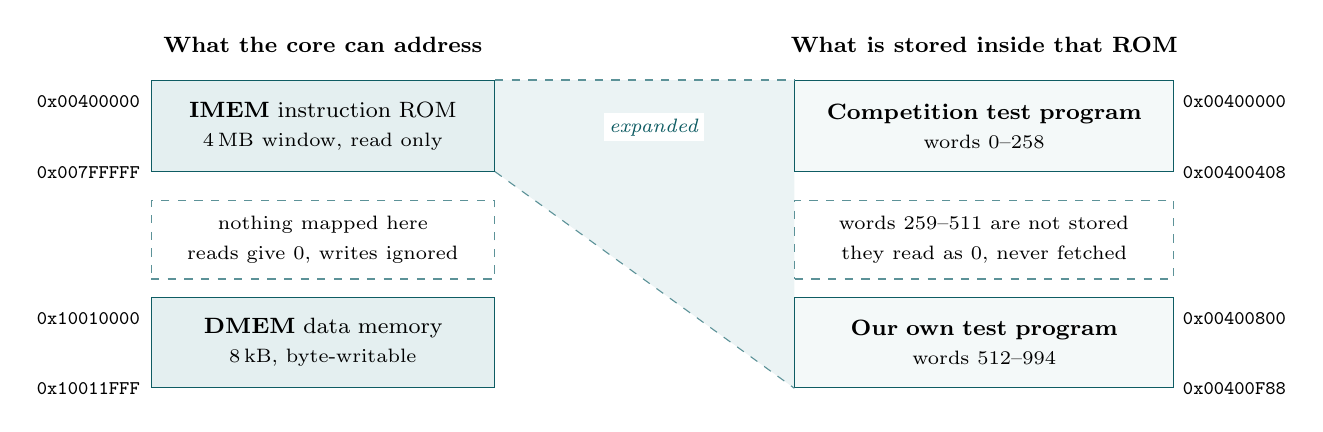
\begin{tikzpicture}[font=\footnotesize,
  reg/.style={draw=rvbl,fill=rvbltint,text width=4.15cm,minimum height=11.5mm,
              align=center,inner sep=3pt},
  rom/.style={draw=rvbl,fill=rvblsoft,text width=4.6cm,minimum height=11.5mm,
              align=center,inner sep=3pt},
  gap/.style={draw=rvblrule,fill=white,text width=4.15cm,minimum height=10mm,
              align=center,inner sep=3pt,dashed},
  romgap/.style={draw=rvblrule,fill=white,text width=4.6cm,minimum height=10mm,
              align=center,inner sep=3pt,dashed},
  adr/.style={font=\scriptsize\ttfamily},
  hd/.style={font=\footnotesize\bfseries}]

% ---------------- left column: the address space the core sees --------------
\node[hd] at (0,1.55) {What the core can address};
\node[reg,anchor=north] (imem) at (0,1.1)
  {\textbf{IMEM} instruction ROM\\[1pt]\scriptsize 4\,MB window, read only};
\node[adr,anchor=east] at (-2.2,0.82) {0x00400000};
\node[adr,anchor=east] at (-2.2,-0.07) {0x007FFFFF};
\node[gap,anchor=north] (hole) at (0,-0.42)
  {\scriptsize nothing mapped here\\[1pt]reads give 0, writes ignored};
\node[reg,anchor=north] (dmem) at (0,-1.65)
  {\textbf{DMEM} data memory\\[1pt]\scriptsize 8\,kB, byte-writable};
\node[adr,anchor=east] at (-2.2,-1.93) {0x10010000};
\node[adr,anchor=east] at (-2.2,-2.82) {0x10011FFF};

% ---------------- right column: what is inside the ROM ----------------------
\node[hd] at (8.4,1.55) {What is stored inside that ROM};
\node[rom,anchor=north] (fw) at (8.4,1.1)
  {\textbf{Competition test program}\\[1pt]\scriptsize words 0--258};
\node[adr,anchor=west] at (10.8,0.82) {0x00400000};
\node[adr,anchor=west] at (10.8,-0.07) {0x00400408};
\node[romgap,anchor=north] (romgap) at (8.4,-0.42)
  {\scriptsize words 259--511 are not stored\\[1pt]they read as 0, never fetched};
\node[rom,anchor=north] (supp) at (8.4,-1.65)
  {\textbf{Our own test program}\\[1pt]\scriptsize words 512--994};
\node[adr,anchor=west] at (10.8,-1.93) {0x00400800};
\node[adr,anchor=west] at (10.8,-2.82) {0x00400F88};

% ---------------- zoom wedge: the right column expands the IMEM box --------
\begin{scope}[on background layer]
  \fill[rvbltint,opacity=0.75]
    (imem.north east) -- (fw.north west) -- (supp.south west) -- (imem.south east) -- cycle;
\end{scope}
\draw[rvblrule,dashed,thin] (imem.north east) -- (fw.north west);
\draw[rvblrule,dashed,thin] (imem.south east) -- (supp.south west);
\node[font=\scriptsize\itshape,rvbl,fill=white,inner sep=2pt,rotate=0]
  at (4.2,0.5) {expanded};

\end{tikzpicture}
\caption{The memory map, and the two programs held in the instruction ROM. The core reads
instructions from one 4\,MB window and reads and writes data in a separate 8\,kB window.
Addresses outside both windows are safe: they read as zero and ignore writes. The shaded
wedge shows that the right-hand column is an expanded view of the ROM only. The ROM stores
742 words, which is 259 words of the competition test program plus 483 words of our own test
program. The 253 words between the two programs are not stored at all and always read as
zero. The competition program must start at the reset address, because it calculates its own
data-memory base from the program counter and therefore cannot be moved. Our own program
does not do this, so it sits above.}
\label{fig:memmap}
\end{figure}

\begin{figure}[htbp]
\centering
% The drawing is a little wider than the text block. Centre it in a zero-width
% box so it bleeds evenly into both margins instead of reporting an overfull
% line and hanging off the right edge only.
\makebox[\linewidth][c]{%
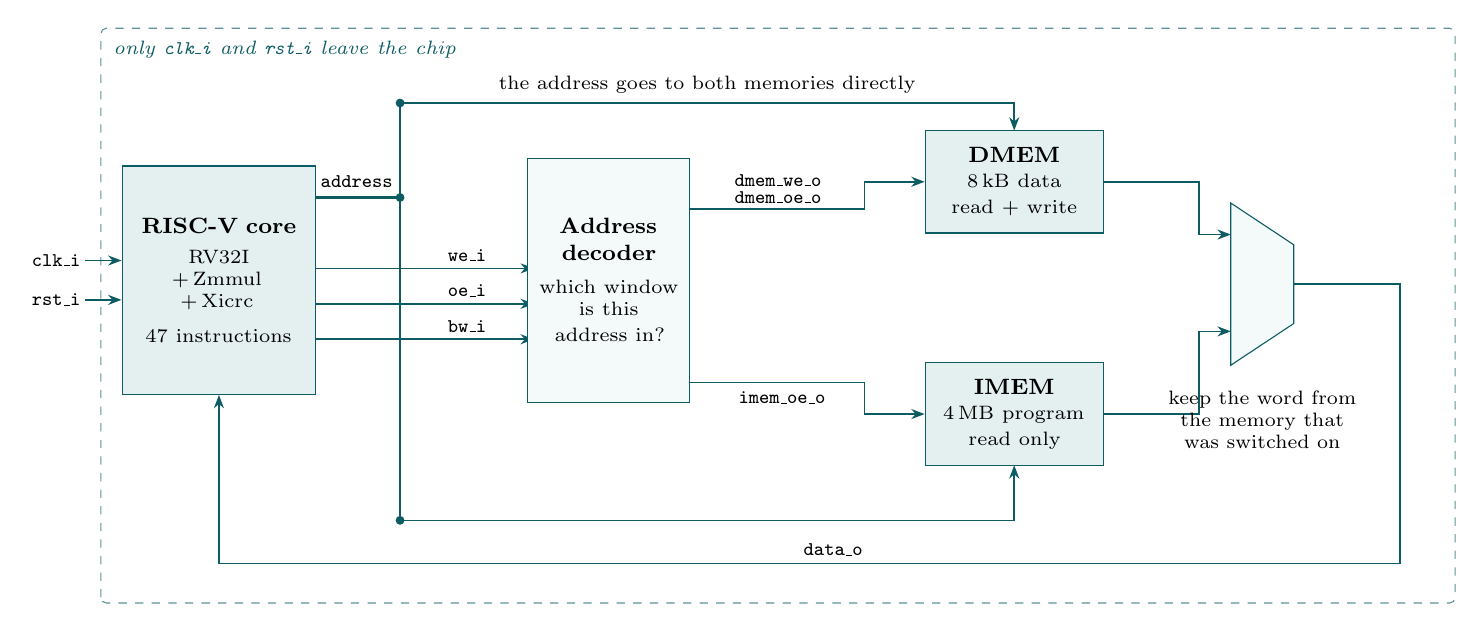
\begin{tikzpicture}[font=\footnotesize,
  core/.style={draw=rvbl,fill=rvbltint,text width=2.25cm,minimum height=2.9cm,
               align=center,inner sep=3pt},
  dec/.style={draw=rvbl,fill=rvblsoft,text width=1.85cm,minimum height=3.1cm,
              align=center,inner sep=3pt},
  mem/.style={draw=rvbl,fill=rvbltint,text width=2.05cm,minimum height=1.3cm,
              align=center,inner sep=3pt},
  sig/.style={font=\scriptsize\ttfamily,inner sep=1.5pt},
  cmt/.style={font=\scriptsize,inner sep=1.5pt},
  w/.style={-{Stealth[length=1.7mm]},rvbl,semithick},
  trunk/.style={rvbl,line width=1.0pt}]

% ---------------- chip outline ---------------------------------------------
\draw[draw=rvblrule,dashed,rounded corners=2pt] (-7.1,-4.0) rectangle (10.1,3.3);
\node[cmt,rvbl,anchor=north west] at (-7.0,3.2)
  {\itshape only \texttt{clk\_i} and \texttt{rst\_i} leave the chip};

% ---------------- pins and core --------------------------------------------
\node[sig,anchor=east] (clk) at (-7.3,0.35) {clk\_i};
\node[sig,anchor=east] (rst) at (-7.3,-0.15) {rst\_i};
\node[core] (cpu) at (-5.6,0.1)
  {\textbf{RISC-V core}\\[3pt]\scriptsize RV32I\\ +\,Zmmul\\ +\,Xicrc\\[3pt]
   \scriptsize 47 instructions};
\draw[w] (clk.east) -- (clk -| cpu.west);
\draw[w] (rst.east) -- (rst -| cpu.west);

% ---------------- trunk: address and the data to be written ----------------
\draw[trunk] (cpu.east |- 0,1.15) -- (-3.3,1.15);
\draw[trunk] (-3.3,2.35) -- (-3.3,-2.95);
\foreach \y in {2.35,1.15,-2.95} \fill[rvbl] (-3.3,\y) circle (1.6pt);
\node[sig,anchor=south] at (-3.85,1.22) {address};

\draw[w] (-3.3,2.35) -- (4.5,2.35) -- (4.5,2.0);
\draw[w] (-3.3,-2.95) -- (4.5,-2.95) -- (4.5,-2.25);
\node[cmt,anchor=south] at (0.6,2.42) {the address goes to both memories directly};

% ---------------- the three strobes into the decoder -----------------------
\foreach \y/\n in {0.25/we\_i, -0.2/oe\_i, -0.65/bw\_i}{
  \draw[w] (cpu.east |- 0,\y) -- (-1.6,\y);
  \node[sig,anchor=south] at (-2.45,\y+0.03) {\n};
}

% ---------------- decoder ---------------------------------------------------
\node[dec] (dec) at (-0.65,0.1)
  {\textbf{Address}\\\textbf{decoder}\\[4pt]\scriptsize which window\\ is this\\ address in?};

% ---------------- memories --------------------------------------------------
\node[mem] (dmem) at (4.5,1.35)  {\textbf{DMEM}\\[1pt]\scriptsize 8\,kB data\\ read + write};
\node[mem] (imem) at (4.5,-1.6) {\textbf{IMEM}\\[1pt]\scriptsize 4\,MB program\\ read only};

\draw[w] (dec.east |- 0,1.0) -- (2.6,1.0) -- (2.6,1.35) -- (dmem.west);
\node[sig,anchor=south,align=center] at (1.5,1.02)
  {dmem\_we\_o\\[-2pt]dmem\_oe\_o};
\draw[w] (dec.east |- 0,-1.2) -- (2.6,-1.2) -- (2.6,-1.6) -- (imem.west);
\node[sig,anchor=north] at (1.55,-1.26) {imem\_oe\_o};

% ---------------- read data returns through the selecting multiplexer ------
\draw[w] (dmem.east) -- (6.85,1.35) -- (6.85,0.68) -- (7.25,0.68);
\draw[w] (imem.east) -- (6.85,-1.6) -- (6.85,-0.55) -- (7.25,-0.55);

\draw[draw=rvbl,fill=rvblsoft] (7.25,1.08) -- (8.05,0.55) -- (8.05,-0.45)
      -- (7.25,-0.98) -- cycle;
\node[cmt,anchor=north,align=center] at (7.65,-1.25) {keep the word from\\ the memory
  that\\ was switched on};

\draw[w] (8.05,0.05) -- (9.4,0.05) -- (9.4,-3.5) -- (cpu.south |- 0,-3.5) -- (cpu.south);
\node[sig,anchor=south] at (2.2,-3.46) {data\_o};

\end{tikzpicture}}
\caption{How the parts are connected. The core makes one memory request at a time. It sends
an address, the data to be written, a read strobe (\texttt{oe\_i}), a write strobe
(\texttt{we\_i}) and four byte-enables (\texttt{bw\_i}). The address decoder compares the
address against the two windows of Figure~\ref{fig:memmap} and switches on no more than one
memory. It switches DMEM on for a read or a write, but IMEM only for a read, because the
program memory has no write port. The decoder then keeps the word from the memory it switched
on and sends it back to the core as \texttt{data\_o}. If the address is in neither window,
the decoder switches on neither memory and returns zero, so a wrong address cannot damage
stored data. Two details differ from a textbook drawing: the address reaches the memories
directly instead of passing through the decoder, and the multiplexer drawn on the right is
part of the address decoder block, not a block of its own.}
\label{fig:soc}
\end{figure}


% =============================================================================
% 2 SUPPORTED INSTRUCTIONS
% =============================================================================
\section{Supported Instructions}
\label{sec:isa}

\textbf{In one paragraph.} The Submission Guide names ten instruction categories. Together
they contain 47 instructions. All 47 are implemented. Each one has a directed test that
passes. Table~\ref{tab:coverage} is the coverage summary in the form the Guide asks for. It
also lists the instructions in each category. Table~\ref{tab:encoding} gives the bit pattern
of every instruction.

\begin{table}[htbp]
\centering\small
\caption{ISA coverage summary with the instructions implemented in each category.
The expected counts come from the Submission Guide (\S2). The implemented counts are what
the control unit block decodes. A passing test covers each one.}
\label{tab:coverage}
\begin{tabularx}{\linewidth}{>{\raggedright\arraybackslash}p{3.5cm}ccc>{\raggedright\arraybackslash}X}
\toprule
\hrow \hdr{Category} & \hdr{Exp.} & \hdr{Impl.} & \hdr{Cov.} & \hdr{Instructions implemented} \\
\midrule
Arith./Logic (Register)  & 10 & 10 & 100\,\% & \texttt{ADD, SUB, SLL, SLT, SLTU, XOR, SRL, SRA, OR, AND} \\
Arith./Logic (Immediate) &  9 &  9 & 100\,\% & \texttt{ADDI, SLTI, SLTIU, XORI, ORI, ANDI, SLLI, SRLI, SRAI} \\
Load                     &  5 &  5 & 100\,\% & \texttt{LB, LH, LW, LBU, LHU} \\
Store                    &  3 &  3 & 100\,\% & \texttt{SB, SH, SW} \\
Branch                   &  6 &  6 & 100\,\% & \texttt{BEQ, BNE, BLT, BGE, BLTU, BGEU} \\
Jump                     &  2 &  2 & 100\,\% & \texttt{JAL, JALR} \\
Upper Immediate          &  2 &  2 & 100\,\% & \texttt{LUI, AUIPC} \\
System / Synchronization &  3 &  3 & 100\,\% & \texttt{ECALL, EBREAK, FENCE} \\
Multiplication (Zmmul)   &  4 &  4 & 100\,\% & \texttt{MUL, MULH, MULHSU, MULHU} \\
CRC (Xicrc)              &  3 &  3 & 100\,\% & \texttt{CRCB, CRCH, CRCW} \\
\midrule
\hrow \textbf{Total} & \textbf{47} & \textbf{47} & \textbf{100\,\%} & \\
\bottomrule
\end{tabularx}
\end{table}

\subsection{Encoding of every implemented instruction}

R-type values come from the Block Guide (Tables 7--9); I/S/B/U/J values are the public
RV32I base encodings. Every row was cross-checked against the decode \texttt{case}
statements in \texttt{control\_unit.v}. This table is what the hardware matches on, not a
separate statement of intent. Note that all seven R-type families share opcode
\texttt{0110011} and are disambiguated by \texttt{funct7} alone
(\texttt{0000000}/\texttt{0100000} base ALU, \texttt{0000001} Zmmul, \texttt{1000000}
Xicrc), which is why the decoder is a two-level structure rather than a 47-way lookup.

\begin{table}[htbp]
\centering\scriptsize
\caption{Full encoding table for all 47 implemented instructions
(Submission Guide \S2). Every row was read back from the decode logic in the control
unit block, so the table shows what the hardware matches on, not what was intended.}
\label{tab:encoding}
\setlength{\tabcolsep}{4pt}
\begin{tabular}{rlcccc<{\hspace{0.75em}}>{\hspace{0.75em}}rlcccc}
\toprule
\hrow \# & \hdr{Instr.} & \hdr{Type} & \hdr{Opcode} & \hdr{f3} & \hdr{funct7} &
\# & \hdr{Instr.} & \hdr{Type} & \hdr{Opcode} & \hdr{f3} & \hdr{funct7} \\
\midrule
 1 & ADD    & R & 0110011 & 000 & 0000000 & 25 & SB     & S & 0100011 & 000 & n/a \\
 2 & SUB    & R & 0110011 & 000 & 0100000 & 26 & SH     & S & 0100011 & 001 & n/a \\
 3 & SLL    & R & 0110011 & 001 & 0000000 & 27 & SW     & S & 0100011 & 010 & n/a \\
 4 & SLT    & R & 0110011 & 010 & 0000000 & 28 & BEQ    & B & 1100011 & 000 & n/a \\
 5 & SLTU   & R & 0110011 & 011 & 0000000 & 29 & BNE    & B & 1100011 & 001 & n/a \\
 6 & XOR    & R & 0110011 & 100 & 0000000 & 30 & BLT    & B & 1100011 & 100 & n/a \\
 7 & SRL    & R & 0110011 & 101 & 0000000 & 31 & BGE    & B & 1100011 & 101 & n/a \\
 8 & SRA    & R & 0110011 & 101 & 0100000 & 32 & BLTU   & B & 1100011 & 110 & n/a \\
 9 & OR     & R & 0110011 & 110 & 0000000 & 33 & BGEU   & B & 1100011 & 111 & n/a \\
10 & AND    & R & 0110011 & 111 & 0000000 & 34 & JAL    & J & 1101111 & n/a & n/a \\
11 & ADDI   & I & 0010011 & 000 & n/a     & 35 & JALR   & I & 1100111 & 000 & n/a \\
12 & SLTI   & I & 0010011 & 010 & n/a     & 36 & LUI    & U & 0110111 & n/a & n/a \\
13 & SLTIU  & I & 0010011 & 011 & n/a     & 37 & AUIPC  & U & 0010111 & n/a & n/a \\
14 & XORI   & I & 0010011 & 100 & n/a     & 38 & ECALL  & I & 1110011 & 000 & \texttt{imm}=0x000 \\
15 & ORI    & I & 0010011 & 110 & n/a     & 39 & EBREAK & I & 1110011 & 000 & \texttt{imm}=0x001 \\
16 & ANDI   & I & 0010011 & 111 & n/a     & 40 & FENCE  & I & 0001111 & 000 & NOP \\
17 & SLLI   & I & 0010011 & 001 & 0000000$^\dagger$ & 41 & MUL    & R & 0110011 & 000 & 0000001 \\
18 & SRLI   & I & 0010011 & 101 & 0000000$^\dagger$ & 42 & MULH   & R & 0110011 & 001 & 0000001 \\
19 & SRAI   & I & 0010011 & 101 & 0100000$^\dagger$ & 43 & MULHSU & R & 0110011 & 010 & 0000001 \\
20 & LB     & I & 0000011 & 000 & n/a     & 44 & MULHU  & R & 0110011 & 011 & 0000001 \\
21 & LH     & I & 0000011 & 001 & n/a     & 45 & CRCB   & R & 0110011 & 000 & 1000000 \\
22 & LW     & I & 0000011 & 010 & n/a     & 46 & CRCH   & R & 0110011 & 001 & 1000000 \\
23 & LBU    & I & 0000011 & 100 & n/a     & 47 & CRCW   & R & 0110011 & 010 & 1000000 \\
24 & LHU    & I & 0000011 & 101 & n/a     &    &        &   &         &     & \\
\bottomrule
\multicolumn{12}{l}{\scriptsize $^\dagger$ occupies \texttt{imm[11:5]}, not a true
\texttt{funct7} field; the decoder requires exactly these values, so
\texttt{SLLI}/\texttt{SRLI}/\texttt{SRAI} with any other} \\
\multicolumn{12}{l}{\scriptsize \phantom{$^\dagger$} value in that field fall through
to the illegal/no-operation default.}
\end{tabular}
\end{table}

\subsection{How coverage was established}

The claim is not that the decoder \emph{contains} 47 cases; it is that all 47 execute
correctly. Three independent mechanisms establish that:

\begin{itemize}
\item \textbf{58 signature tests} in \texttt{tb\_firmware} compute
  \texttt{actual XOR expected} into a dedicated data-memory word per test, with every
  expected value computed independently in Python rather than by the RTL. There are 58
  rather than 47 because loads and stores are tested at \emph{every} byte lane
  (\texttt{address[1:0]} = 0/1/2/3) and every branch condition is tested in both the taken
  and the not-taken direction. \texttt{JAL}, \texttt{JALR}, \texttt{AUIPC},
  \texttt{FENCE}, \texttt{ECALL} and \texttt{EBREAK}, which produce no comparable register
  result, are checked structurally.
\item \textbf{A complete decode sweep} drives 704 different instruction encodings through
  the real state machine. Invalid encodings are included on purpose. Each one is checked
  twice: which state follows \textsc{execute}, and whether the register write is enabled.
  The expected answers come from a separate model written from the instruction tables. That
  model was not copied from the design.
\item \textbf{The organisers' own validation firmware}, which exercises RV32I, all four
  multiplies and all three CRC widths and returns \texttt{x4 = 0} (\S\ref{sec:firmware}).
\end{itemize}


% =============================================================================
% 3 DATAPATH
% =============================================================================
\section{Datapath and Control Unit}
\label{sec:datapath}

\textbf{In one paragraph.} Figure~\ref{fig:datapath} shows the complete datapath and the
control unit. Solid lines carry data. Dashed lines are control signals from the
finite-state machine (FSM). Every box is a real block on the ChipInventor canvas, and every
line is a real wire. This is the design itself, not a simplified drawing of it.

Read one point first. The core has only \emph{one} memory port. The FSM shares that port
over time between instruction fetch and data access, and the address decoder sends each
request to the correct memory. This sharing is the reason the Block Guide requires a
multicycle design.

\begin{figure}[htbp]
\centering
\makebox[\linewidth][c]{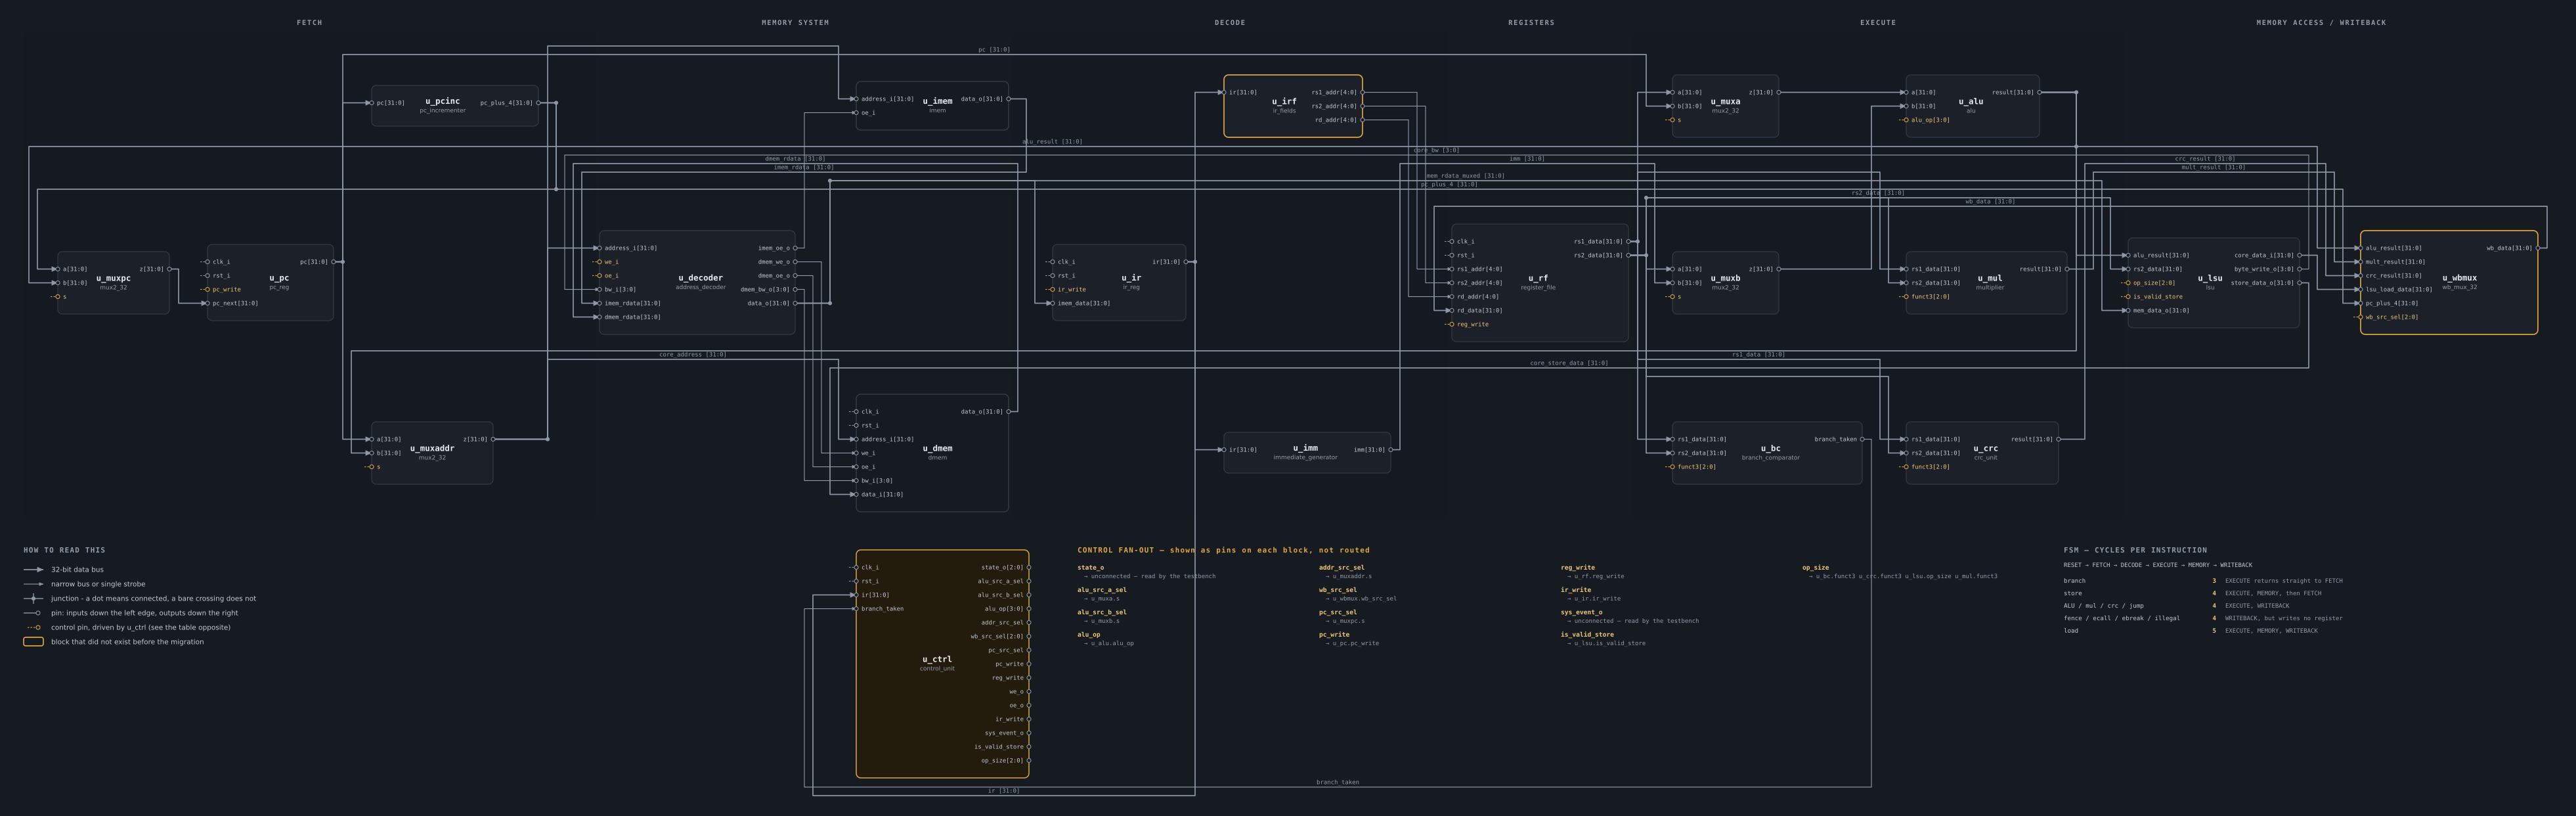
\includegraphics[width=1.13\linewidth]{figures/soc-architecture.png}}
\caption{The complete RVBL-2 datapath and control unit, exported from the design itself.
The columns follow the order of a single instruction, left to right: \textsc{fetch}, the
memory system, \textsc{decode}, the registers, \textsc{execute}, and finally memory access
and \textsc{writeback}. Every box is one of the 20 block instances on the canvas and every
line is one of the 43 nets between them, made from 72 connections. The control unit sits at
the bottom. Its outputs are printed beside it as a list rather than drawn as 15 separate
lines, because each one reaches almost every block above. Three panels at the bottom left
give the drawing key, the control fan-out, and the number of cycles each class of
instruction takes. One ALU serves arithmetic, address calculation and branch targets. One
memory port serves both instruction fetch and data access. The multiplier, the CRC unit and
the branch comparator all calculate during \textsc{execute}, every time; their answers are
simply not selected when they are not wanted. \textbf{This diagram is dense on purpose: it
is the design itself, not a simplification. Zoom in to read the signal names.}}
\label{fig:datapath}
\fullresbar{soc-architecture.png}
\end{figure}

\subsection{Control unit: the finite-state machine}

Block Guide \S3.2 names four phases. This design uses six states: the four named phases,
plus \textsc{reset}, plus a \textsc{memory} state. The \textsc{memory} state is not
decoration. Block Guide \S4.3 specifies the data memory as synchronous
(``the operation will only be completed after a clock cycle''), so a load physically cannot
present an address and consume the result in the same cycle. Six states encode in three
bits, so the addition costs nothing.

\begin{figure}[htbp]
\centering
\begin{minipage}{0.615\linewidth}
\centering
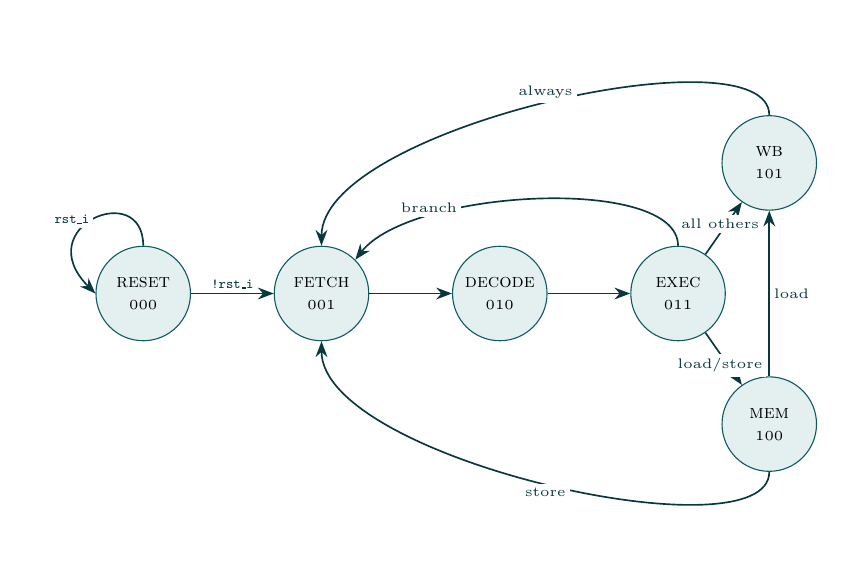
\begin{tikzpicture}[font=\scriptsize,>=Stealth,node distance=10.5mm,
  st/.style={draw=rvbl,fill=rvbltint,circle,minimum size=12mm,align=center,inner sep=0pt},
  ed/.style={->,rvbldark,semithick},
  lb/.style={font=\tiny,inner sep=1.5pt,fill=white}]
\node[st] (rst) {\textsc{reset}\\\tiny 000};
\node[st,right=of rst] (f) {\textsc{fetch}\\\tiny 001};
\node[st,right=of f] (d) {\textsc{decode}\\\tiny 010};
\node[st,right=of d] (e) {\textsc{exec}\\\tiny 011};
\node[st,below right=8mm and 3mm of e] (m) {\textsc{mem}\\\tiny 100};
\node[st,above right=8mm and 3mm of e] (w) {\textsc{wb}\\\tiny 101};

\draw[ed] (rst) -- node[lb,above]{\texttt{!rst\_i}} (f);
\draw[ed] (f) -- (d);
\draw[ed] (d) -- (e);
\draw[ed] (e) -- node[lb,below,pos=0.4]{load/store} (m);
\draw[ed] (e) -- node[lb,above,pos=0.4]{all others} (w);
\draw[ed] (m) -- node[lb,right,pos=0.5]{load} (w);
\draw[ed] (m.south) .. controls +(0,-1.1) and +(0,-1.5) .. node[lb,below]{store} (f.south);
% Every transition carries a condition, so this one is labelled too. Note
% that an EMPTY node here would still paint lb's white fill and cut the arc.
\draw[ed] (w.north) .. controls +(0,1.1) and +(0,1.5) ..
  node[lb,above,pos=0.5]{always} (f.north);
\draw[ed] (e.north) .. controls +(0,0.9) and +(0.7,0.9) ..
  node[lb,above,pos=0.75]{branch} (f.north east);
\draw[ed] (rst.north) .. controls +(0,0.85) and +(-0.85,0.85) ..
  node[lb,left,pos=0.5]{\texttt{rst\_i}} (rst.west);
\end{tikzpicture}
\end{minipage}\hfill
\begin{minipage}{0.37\linewidth}
\scriptsize
\begin{tabularx}{\linewidth}{Xr}
\toprule
\hrow \hdr{Instruction class} & \hdr{Cycles} \\
\midrule
Branch (taken or not)                       & 3 \\
Store (\texttt{SB}/\texttt{SH}/\texttt{SW}) & 4 \\
ALU-reg, ALU-imm, \texttt{LUI},
\texttt{AUIPC}, \texttt{MUL}$*$,
\texttt{CRC}$*$, \texttt{JAL},
\texttt{JALR}, \texttt{FENCE},
\texttt{ECALL}/\texttt{EBREAK}, illegal     & 4 \\
Load (all five widths)                      & 5 \\
\bottomrule
\end{tabularx}
\vspace{3pt}
{\tiny This table is the control unit's own next-state logic. It was verified by 53
directed transition checks, and by driving all 704 possible instruction encodings through
the real state machine.}
\end{minipage}
\caption{Control-unit FSM: six states, 3-bit binary encoding, and the resulting cycle count
per instruction class. \texttt{rst\_i} is synchronous and additionally gates every
combinational control output directly, so an in-flight store's write enable drops in the
\emph{same} cycle reset asserts rather than one cycle later, confirmed at SoC level by
injecting reset at 40 different points of a running program and checking that no data-memory
word changed across the reset edge.}
\label{fig:fsm}
\end{figure}

\subsection{Control signals and datapath multiplexers}

The control unit produces every select signal in the datapath. Table~\ref{tab:mux} lists
each multiplexer, the values it can choose between, and the signal that makes the choice.
Four of the five multiplexers choose between two values. The writeback multiplexer chooses
between five, because five different units can produce a register result. One signal,
\texttt{op\_size}, is not a select at all: it is \texttt{funct3} republished by the control
unit so that four blocks read the width field from one source instead of four.

\begin{table}[htbp]
\centering\scriptsize
\caption{Every multiplexer in the datapath, what it can choose between, and which signal
makes the choice. The control unit drives all of these selects. The program-counter select
also depends on \texttt{branch\_taken} in the same cycle. This is deliberate, and it is what
lets a branch finish in three cycles.}
\label{tab:mux}
\setlength{\tabcolsep}{5pt}
\begin{tabularx}{\linewidth}{llXX}
\toprule
\hrow \hdr{Mux (instance)} & \hdr{Select} & \hdr{Sources} & \hdr{Purpose} \\
\midrule
\texttt{u\_muxa}    & \texttt{alu\_src\_a\_sel} & \texttt{rs1\_data} $\mid$ \texttt{pc} &
  ALU operand A; \texttt{pc} for \texttt{AUIPC} and branch/\texttt{JAL} target math \\
\texttt{u\_muxb}    & \texttt{alu\_src\_b\_sel} & \texttt{rs2\_data} $\mid$ \texttt{imm} &
  ALU operand B; immediate for every I/S/B/U/J format \\
\texttt{u\_muxaddr} & \texttt{addr\_src\_sel}   & \texttt{pc} $\mid$ \texttt{alu\_result} &
  Shared memory address: \texttt{pc} during fetch, effective address during
  \textsc{execute}/\textsc{memory}, \emph{and through \textsc{writeback} for loads} \\
\texttt{u\_muxpc}   & \texttt{pc\_src\_sel}     & \texttt{pc\_plus\_4} $\mid$
  \texttt{alu\_result} & Next PC; target when a branch is taken or on \texttt{JAL}/\texttt{JALR} \\
\texttt{u\_wbmux}   & \texttt{wb\_src\_sel[2:0]} & \texttt{alu\_result} $\mid$
  \texttt{mult\_result} $\mid$ \texttt{crc\_result} $\mid$ \texttt{lsu\_load\_data} $\mid$
  \texttt{pc\_plus\_4} & Register-file write data \\
n/a & \texttt{alu\_op[3:0]} & 11 operations, Block Guide Table 9 (\texttt{4'h0} \texttt{PASS\_B}
  $\ldots$ \texttt{4'hA} \texttt{SLTU}) & ALU function select \\
n/a & \texttt{op\_size[2:0]} & \texttt{funct3}, republished by the control unit & Drives
  \texttt{branch\_comparator}, \texttt{multiplier}, \texttt{crc\_unit} and \texttt{lsu}
  from one source \\
\bottomrule
\end{tabularx}
\end{table}

\begin{callout}{One timing detail: a load that reads from the program memory}
The Block Guide (\S4.2) permits a \texttt{LW} to read from a program-memory address. Programs
use this to read constants that they store between their instructions. The competition
firmware does it twice. It reads its CRC test data from \texttt{0x004003F8} and its copy-loop
source data from \texttt{0x00400400}.

The two memories behave differently, and this matters. The data memory has an output
register, so it holds the word it read. The program memory has no output register. Its
output follows its enable immediately.

If the read enable went low at the start of \textsc{writeback}, the program memory output
would fall to zero in that same cycle. The register file samples the value in exactly that
cycle. The load would then write zero, and nothing would report an error.

The fix is to keep the read enable and the address selection at their \textsc{execute}
values through \textsc{writeback}, but only for loads. This costs no extra register. It has
no effect on data-memory loads.

Stores are different. A store has no \textsc{writeback} cycle, and its write enable must go
low before the address changes. The write enable is therefore limited to \textsc{memory}.
This difference between loads and stores is deliberate. Validation stage 7 confirms the
behaviour on the complete system.
\end{callout}


% =============================================================================
% 4 MODULES AND TESTBENCHES
% =============================================================================
\section{Modules and Testbenches}
\label{sec:modules}

\textbf{In one paragraph.} On the ChipInventor canvas the processor is
\textbf{17 block definitions}. These are placed as \textbf{20 instances} and joined by
\textbf{72 connections}, which form \textbf{45 nets}. The top level has exactly
\textbf{2 pins}. Each block is a unit that can be tested on its own, and each has its own
directed testbench.

This section gives four things: the interface and role of every block, the testbench that
covers it, how the blocks are connected on the platform, and the twelve automatic gates that
must pass before anything is pasted into ChipInventor.

\vspace{2pt}
{\small
\begin{tabularx}{\linewidth}{>{\raggedright\arraybackslash}p{5.3cm}rX}
\toprule
\hrow \hdr{Evidence} & \hdr{Measured} & \hdr{What it demonstrates} \\
\midrule
Block definitions on the canvas & 17 & Each one verified on its own \\
Instances, and nets between them & 20 / 45 & 72 connections, 2 top-level pins \\
Reference regression, block level & 7{,}384 & 15 testbenches, 0 failures \\
\quad with the gate-level testbench & 8{,}285 & 16 testbenches, needs Yosys \\
Platform suite, one pasted file & \textbf{15{,}281} & 5 suites, 0 failures \\
Automatic gates before submission & 12 & All pass, see Listing~\ref{lst:gates} \\
Mirror equivalence, cycle by cycle & 410{,}400 & 0 mismatches against the
  reference design \\
Competition firmware verdict & \ok & \texttt{x4 = 0x00000000} after 991 cycles \\
\bottomrule
\end{tabularx}}

\vspace{2pt}
{\footnotesize The two suites are independent. The reference regression tests the design as
sixteen separate files. The platform suite tests the single file that ChipInventor actually
runs. A fault would have to appear in both to pass unnoticed.}





\subsection{Per-module implementation and its testbench}

% The caption is issued FIRST so that \thetable is already incremented when the
% two sub-table headers below typeset "Table <n>a" and "Table <n>b".
\begin{minipage}{\linewidth}
\captionof{table}{The 17 canvas blocks: interface width, role, and the testbench that
verifies each. ``Checks'' is the count from the standalone regression run reproduced for
this report; blocks marked \emph{glue} are covered by suite S0.11 of the platform testbench
and indirectly by every integration test.}
\label{tab:modules}
\vspace{3pt}

{\footnotesize
\begin{tabularx}{\linewidth}{>{\ttfamily\scriptsize}p{2.05cm}c>{\raggedright\arraybackslash}X>{\raggedright\arraybackslash}p{4.35cm}r}
\multicolumn{5}{l}{\normalsize\bfseries\color{rvbl}Table \thetable a\quad
  Control and instruction-issue blocks}\\[2pt]
\toprule
\hrow \normalfont\bfseries Block & \bfseries In/Out & \bfseries Role &
\bfseries Testbench & \bfseries Checks \\
\midrule
control\ub unit & 4/15 & 6-state FSM; instruction-class decode on the full
  \texttt{\{opcode,funct3,funct7\}} tuple; emits every control signal &
  \texttt{tb\_control\_unit}: 704-encoding sweep, 53 transition-table checks,
  mid-instruction reset abort & 1461 \\
pc\_reg & 4/1 & Program counter; reset vector \texttt{0x00400000}; bits [1:0] forced to 0
  on every load & \texttt{tb\_core}, \texttt{tb\_soc}, \texttt{tb\_reset}; S1.2 & n/a \\
pc\ub incrementer & 1/1 & Dedicated \texttt{PC+4} adder, deliberately not the shared ALU &
  S0.11 \emph{glue}; exercised by every program & n/a \\
ir\_reg & 4/1 & Instruction register; written once per instruction, at the
  \textsc{fetch}$\to$\textsc{decode} edge & S0.11 \emph{glue}; \texttt{tb\_core} & n/a \\
ir\_fields & 1/3 & Extracts \texttt{rs1}/\texttt{rs2}/\texttt{rd} addresses; exists because
  the canvas cannot slice a bus (\S\ref{sec:canvas}) & S0.11 \emph{glue} & n/a \\
immediate\ub generator & 1/1 & I/S/B/U/J immediate extraction and sign extension, purely
  combinational & \texttt{tb\_immediate\_generator}: checked against an independent
  Python bit-slicer & 34 \\
register\ub file & 7/2 & 32\,$\times$\,32-bit GPRs; \texttt{x0} hardwired to zero; 2
  asynchronous reads, 1 synchronous write & \texttt{tb\_register\_file}: \texttt{x0}
  write-guard, full round trip, reset & 36 \\
mux2\_32 ($\times$4) & 3/1 & Generic 2-to-1 32-bit multiplexer; four instances, per
  Table~\ref{tab:mux} & S0.11 \emph{glue} & n/a \\
\bottomrule
\end{tabularx}}
\end{minipage}

\vspace{6pt}

{\footnotesize
\begin{tabularx}{\linewidth}{>{\ttfamily\scriptsize}p{2.05cm}c>{\raggedright\arraybackslash}X>{\raggedright\arraybackslash}p{4.35cm}r}
\multicolumn{5}{l}{\normalsize\bfseries\color{rvbl}Table \thetable b\quad
  Execution, memory and interconnect blocks}\\[2pt]
\toprule
\hrow \normalfont\bfseries Block & \bfseries In/Out & \bfseries Role &
\bfseries Testbench & \bfseries Checks \\
\midrule
alu & 3/1 & 11 operations exactly per Block Guide Table 9; shift amounts masked to
  \texttt{b[4:0]}; safe \texttt{default} & \texttt{tb\_alu}: directed per-op corners
  (0, $\pm$1, \texttt{INT\_MIN/MAX}, shift $\ge$32) + 1{,}100 randomised & 1128 \\
branch\ub comparator & 3/1 & The 6 RV32I branch conditions, signed/unsigned aware; reserved
  \texttt{funct3} defaults to not-taken & \texttt{tb\_branch\_comparator}: all 6 in both
  directions, signed/unsigned boundary & 24 \\
multiplier & 3/1 & \texttt{MUL}/\texttt{MULH}/\texttt{MULHSU}/\texttt{MULHU},
  combinational 64-bit product, Table 10 & \texttt{tb\_multiplier}: 2{,}198 vs an
  independent 64-bit reference, + 4 truth-table checks of the sign/half formulas & 2202 \\
crc\_unit & 3/1 & CRC-16/CCITT-FALSE over 8/16/32-bit inputs as three constant-width XOR
  networks plus an output mux, per Table 11 & \texttt{tb\_crc\_unit}: independent Python
  bit-serial model, the standard \texttt{0x29B1} check value, the firmware's
  \texttt{0x1E82} anchor & 322 \\
lsu & 5/3 & Byte-lane placement, sign/zero extension, 4-bit byte-write strobe generation &
  \texttt{tb\_lsu}: reproduces the Block Guide's own worked examples exactly, plus a
  full alignment sweep & 26 \\
wb\_mux\_32 & 6/1 & 5-source writeback multiplexer (ALU, multiplier, CRC, load data,
  \texttt{PC+4}) & S0.11 \emph{glue} & n/a \\
address\ub decoder & 6/5 & Memory-mapped routing per Table 13; \texttt{we} never reaches the
  ROM; \texttt{bw} reaches only the SRAM & \texttt{tb\_address\_decoder}: boundary sweep
  \emph{and} out-of-range store asserts zero write enable & 12 \\
imem & 2/1 & 742-word instruction/constant ROM, combinational read, \texttt{oe}-gated &
  \texttt{tb\_imem}: \texttt{oe} gating; out-of-array reads return 0, not an alias & 7 \\
dmem & 7/1 & Synchronous, byte-writable data SRAM; \texttt{DMEM\_WORDS = 2048} (the full
  8\,kB) on the canvas & \texttt{tb\_dmem}: byte lanes, true storage, write-wins,
  implemented-size boundary & 17 \\
\bottomrule
\end{tabularx}}






\vspace{4pt}
Four more testbenches test the assembled system instead of one block. They are
\texttt{tb\_core} (29 checks on the core with the decoder and both memories),
\texttt{tb\_soc} (14 checks on the two-pin top level, including a load from the program
memory), \texttt{tb\_reset} (2{,}002 checks, with reset applied at 40 different points of a
running program) and \texttt{tb\_firmware} (70 checks that reach all 47 instructions through
58 signature tests).

A sixteenth testbench, \texttt{tb\_gatelevel}, compares the design against a synthesised
netlist cycle by cycle for 900 cycles. It needs the Yosys tool. If that tool or its netlist
is absent, the suite skips this testbench. It does not fail it. The run shown in
\S\ref{sec:firmware} is such a run.

\subsection{SoC-level interconnection on the ChipInventor platform}
\label{sec:canvas}

\begin{minipage}[t]{0.52\linewidth}
\vspace{0pt}
The canvas imposes two constraints that shaped the block decomposition, and both are worth
stating because they explain structure that would otherwise look redundant.

\textbf{The canvas cannot cut a bus into pieces.} Each connection joins one complete port
to another complete port of the same width. An exported project contains no partial
connection at all. You therefore cannot draw \texttt{ir[19:15]} as a wire.

This is why \texttt{ir\_fields} is a block of its own. It takes the instruction word and
publishes the three register numbers as separate ports. For the same reason the design
never extracts \texttt{funct3} twice. The control unit publishes it once as
\texttt{op\_size}, and the branch comparator, the multiplier, the CRC unit and the load-store
unit all use that one output. One source cannot disagree with itself.

\textbf{Macros leak between blocks.} The platform joins the source of every block into one
file. A \texttt{`define} in one block is therefore visible in all the others. Every block
here uses \texttt{localparam} instead, which belongs to one module only.

Gate 9 checks this automatically. It also rejects four other constructs: \texttt{`ifdef},
\texttt{`include}, \texttt{\$readmemh} and \texttt{initial} blocks. Each of these fails
\emph{quietly} on a platform that has no file system.
\end{minipage}\hfill
\begin{minipage}[t]{0.44\linewidth}
\vspace{0pt}
\centering\small
\captionof{table}{What a complete RVBL-2 project on the canvas contains. These counts
are recounted automatically from the design before every submission.}
\label{tab:canvas}
\begin{tabularx}{\linewidth}{Xr}
\toprule
\hrow \hdr{Canvas element} & \hdr{Count} \\
\midrule
Block definitions to create   & 17 \\
Block instances to place      & 20 \\
Input pins (\texttt{clk\_i}, \texttt{rst\_i}) & 2 \\
Nets                          & 45 \\
Individual connections to draw & 72 \\
\midrule
Internal wires in the export  & 41 \\
Module definitions in the export & 18 \\
ROM words                     & 742 \\
\bottomrule
\end{tabularx}
\vspace{4pt}
{\scriptsize Two control-unit outputs, \texttt{state\_o} and \texttt{sys\_event\_o}, are
deliberately left unconnected: the top level has only the two pins Block Guide Table 5
mandates, so there is nowhere for them to go. The testbench observes them through
hierarchical references instead. This is why three different net counts appear in this
report, and all three are correct: the canvas checklist has \textbf{45} rows, the exported
netlist has \textbf{43} nets because those two have no destination, and the top module
declares \textbf{41} internal wires because two of the 43 are the input pins themselves.}
\end{minipage}

\subsubsection{A two-pin top level, and how observability was preserved}
\label{sec:observability}

Block Guide Table 5 permits exactly two pins, and both are inputs. The chip therefore has
no data output. This creates a real danger. A synthesis tool removes any logic that cannot
reach an output, so it can delete the whole design. This is not a theory. During development
Yosys did exactly that and reported \textbf{0 cells}.

The defence is to mark the storage elements with \texttt{(* keep *)}. Three are marked: the
data memory array, the register file array, and the state register of the control unit.
Anything that feeds a kept register also survives, so these three marks hold the whole
datapath in place.

One detail about the platform matters here. The platform rebuilds each module header from
its own input and output form fields. A mark on a \emph{port} declaration is therefore lost
in the export, but a mark on an \emph{internal} declaration is kept. Gate 11 lists the three
marks that were lost. It lists them as notes, not failures, because the three kept arrays
already hold those paths.

The cell count proves the defence worked. Synthesis produced \textbf{17{,}708 cells and
1{,}393 flip-flops}. The architecture needs about 1{,}315 flip-flops: 992 for the register
file (31 registers of 32 bits; \texttt{x0} is hardwired and needs none), 256 for the data
memory in this build, 32 for the program counter, 32 for the instruction register and 3 for
the state. Every storage element is present, and nothing was removed.

\figorbox{figures/ci_canvas.png}{0.95\linewidth}
  {ChipInventor canvas screenshot.}
  {The processor as drawn on the ChipInventor canvas. Each white card is one block instance. Each blue line is one wire. There are 20 instances and 72 connections, which together form 45 nets. The two small cards at the bottom left are the only input pins, \texttt{clk\_i} and \texttt{rst\_i}.}
  {fig:canvas}

\figorbox{figures/ci_block_editor.png}{0.86\linewidth}
  {ChipInventor block library.}
  {The block library on the platform, showing 9 of the 17 blocks. Each card gives the block name, the icon the platform generates, and the number of inputs, outputs and bidirectional ports. No block has a bidirectional port. The port counts here match the interface column of Table~\ref{tab:modules} exactly, which confirms that what was entered on the platform is what was verified.}
  {fig:blocklib}

\subsection{The platform testbench and the twelve verification gates}

The platform runs a testbench only at project level. It cannot run one testbench per block.
We therefore combined our sixteen separate testbenches into one file. That file is what we
paste into the platform's testbench field.

The combined testbench creates the project as \texttt{top dut}, connects the clock and the
reset, and then reads the internal signals through hierarchical names. This is the only way
to observe a design that has no data outputs.

Two changes were necessary. The platform has no file system, so the tests cannot read a file
of expected values. Each of those files became a reference function inside the testbench
instead. The functions also sweep more values than the fixed files did.

The combined testbench runs \textbf{15{,}281 checks} in five suites:

\begin{itemize}[leftmargin=1.35em,itemsep=0pt,topsep=2pt]
\item \textbf{S0}, about 9{,}900 checks: each block on its own.
\item \textbf{S1}, about 1{,}500 checks: the control state machine.
\item \textbf{S2A}: the official validation firmware.
\item \textbf{S2B}, about 80 checks: our own coverage program.
\item \textbf{S3}, about 3{,}700 checks: reset applied during a running program.
\end{itemize}

Before anything is pasted, a script runs twelve gates on a local machine. Listing~\ref{lst:gates}
is that script's own output, copied into this report without editing.

\begin{lstlisting}[caption={The twelve verification gates, exactly as the script
printed them. Gates 11 and 12 activate only once the project has been exported from the
platform into the repository, which it has.},label={lst:gates},captionpos=b]
=== 1/12  Official validation firmware is intact ===
OK   official firmware: 259 words, 0x00400000..0x00400408, contiguous, sha256 pinned
=== 2/12  Supplementary firmware image is current ===
OK   position-independent: 483 words identical at 0x00400000 and 0x00400800
=== 3/12  Generated ROM matches both firmware images ===
OK   imem.v: 742 words - validation_firmware.hex @ word 0 (259), ci_prog.hex @ word 512 (483)
=== 4/12  Testbench constants match the firmware ===
OK   official firmware anchors still point at the right instructions (4)
=== 5/12  Mirror equivalence: ci_top.v vs the verified original ===
OK   410400 passed, 0 failed
=== 6/12  Combined suite against the local mirror ===
OK   15281 passed, 0 failed
=== 7/12  OFFICIAL VALIDATION FIRMWARE VERDICT ===
OK   Firmware settled after 991 cycles at pc=004003ec (all_good)
OK   x4 = 00000000 - the official firmware PASSES on this core
=== 8/12  Mock IMEM drives the core (this is what OpenLane synthesises) ===
OK   mock ROM runs on the core: x5=10, x6=5, x7=15
=== 9/12  Blocks are free of constructs the platform cannot resolve ===
OK   no ifdef / include / file I/O in any block
OK   no initial blocks in any block (nothing leaks into synthesis)
=== 10/12  Schematic layout is clean ===
OK   canvas 3923x1242, 20 blocks, 46 routed wires, 12 columns
=== 11/12  Exported netlist matches the verified design ===
     OK   all 17 block sources match blocks/*.v
     OK   ROM is bit-identical to blocks/imem.v (742 words)
     OK   20 instances, same block mix as ci_top.v
     OK   netlist is graph-identical to ci_top.v (43 nets; unconnected in the export:
          control_unit.state_o, control_unit.sys_event_o)
     OK   dmem DMEM_WORDS = 2048
=== 12/12  Combined suite against the EXPORTED netlist ===
OK   15281 passed, 0 failed on the exported netlist
OK   official firmware PASSES on the exported netlist
========================================
 ALL CHECKS PASSED - safe to paste into ChipInventor
========================================
\end{lstlisting}

\figorbox{figures/platform_tb_pass_log.png}{0.94\linewidth}
  {ChipInventor simulation log.}
  {The same testbench running \emph{on the platform}, not on a local simulator. The
   platform's own Simulation Log reports \texttt{15281 passed, 0 failed} and
   \texttt{ALL TESTS PASSED}. The visible lines above the total are the last three checks of
   the reset-stress suite, including the re-run that returns \texttt{x4=00000000} after 991
   cycles. This is the result that matters: the design passes where it will be built.}
  {fig:platformlog}

\subsection{Synthesis and place-and-route on the platform}

\emph{ChipInventor's own} OpenLane installation produced the layout in
\S\ref{sec:openlane}. It used the configuration submitted with this project, and it worked
on the design that the platform itself generated from the canvas.

Two independent facts prove that the platform built this design and not some other one.
First, gate 11 shows that the exported netlist has the same structure as the verified one.
Second, all seventeen blocks in the file the platform generated were compared against the
submitted source. Every one was identical. The top module carries 41 wires with the same
names, the same widths and the same order.

\figorbox{figures/ci_run.png}{0.92\linewidth}
  {ChipInventor layout viewer.}
  {The finished layout opened in the ChipInventor layout viewer. The panel on the right lists the Sky130 mask layers that the GDSII file contains, from the wells and diffusion up through the metal layers. The scale bar at the bottom left reads 100\,\textmu m. This is the platform showing its own result, not a local copy.}
  {fig:cirun}


% =============================================================================
% 5 OPENLANE RESULTS
% =============================================================================
\section{OpenLane Results}
\label{sec:openlane}

\textbf{In one paragraph.} The design was taken from Verilog to GDSII by OpenLane on the
ChipInventor platform, targeting SkyWater sky130A with the \texttt{sky130\_fd\_sc\_hd}
standard-cell library and \emph{no} hard macros. The flow completed with zero design-rule
violations, zero routing violations, a layout-versus-schematic match that is unique, and
positive setup and hold margin at all three timing corners. Table~\ref{tab:area} is the
area and density result the Submission Guide asks for; Figure~\ref{fig:gds} is the final
GDSII.

\begin{figure}[htbp]
\centering
\begin{tikzpicture}[font=\scriptsize,>=Stealth,
  s/.style={draw=rvbl,fill=rvbltint,rounded corners=1.5pt,minimum height=8mm,
            text width=1.72cm,align=center,inner sep=2pt},
  g/.style={font=\tiny,align=center,text width=1.85cm,color=okgreen},
  a/.style={->,rvbl,semithick}]
\node[s] (sy) at (0,0)    {Synthesis\\\tiny Yosys + ABC};
\node[s] (fp) at (2.1,0)  {Floorplan\\\tiny + PDN};
\node[s] (pl) at (4.2,0)  {Placement};
\node[s] (ct) at (6.3,0)  {CTS};
\node[s] (rt) at (8.4,0)  {Routing\\\tiny global + detail};
\node[s] (sg) at (10.5,0) {Signoff\\\tiny DRC/LVS/STA};
\node[s,fill=rvbl!22] (gd) at (12.6,0) {\textbf{GDSII}};
\foreach \a/\b in {sy/fp,fp/pl,pl/ct,ct/rt,rt/sg,sg/gd} \draw[a] (\a) -- (\b);
\node[g,below=2.5mm of sy] {17{,}708 cells\\1{,}393 flops\\\emph{not swept}};
\node[g,below=2.5mm of fp] {core 618.7\\$\times$\,617.44\,\textmu m\\\emph{config applied}};
\node[g,below=2.5mm of pl] {no DPL-0035\\no DPL-0036};
\node[g,below=2.5mm of ct] {clock tree\\on \texttt{clk\_i}};
\node[g,below=2.5mm of rt] {\textbf{0} routing\\violations};
\node[g,below=2.5mm of sg] {\textbf{0} DRC \textbullet{} LVS\\unique \textbullet{}
  +2.25\,ns};
\node[g,below=2.5mm of gd] {0.404\,mm$^2$\\51\,MB};
\end{tikzpicture}
\caption{The OpenLane flow, and the check applied at each stage. ``Did the flow finish'' is
the wrong question, for two reasons. First, a two-pin design can be reduced to nothing and
still pass every later stage. Second, OpenLane does \emph{not} stop for a timing violation.
It returns a complete layout that simply misses its clock target. We therefore checked each
gate above on its own. Every result in Table~\ref{tab:signoff} was read from the report file
the tool wrote.}
\label{fig:olflow}
\end{figure}

\begin{table}[htbp]
\begin{minipage}[t]{0.485\linewidth}
\vspace{0pt}\centering\small
\captionof{table}{Total area and density after physical implementation (Submission Guide
\S5). Every figure is taken from the run's own metrics report.}
\label{tab:area}
\begin{tabularx}{\linewidth}{Xr}
\toprule
\hrow \hdr{Metric} & \hdr{Value} \\
\midrule
Die dimensions            & 630.15 $\times$ 640.87 \textmu m \\
\textbf{Total die area}   & \textbf{0.4038 mm$^2$} \\
Core dimensions           & 618.70 $\times$ 617.44 \textmu m \\
Core area                 & 382{,}010 \textmu m$^2$ \\
Standard-cell area        & 191{,}649 \textmu m$^2$ \\
\textbf{Final utilisation (density)} & \textbf{52.28\,\%} \\
Cell density              & 47{,}786 cells/mm$^2$ \\
\midrule
Standard cells            & 17{,}708 \\
Flip-flops                & 1{,}393 \\
Total placed instances    & 51{,}267 \\
\quad decap / fill / well-tap & 17{,}132 / 8{,}940 / 5{,}381 \\
\quad antenna diodes      & 516 \\
Total wirelength          & 869{,}840 \textmu m (0.87 m) \\
Vias                      & 151{,}445 \\
\bottomrule
\end{tabularx}
\end{minipage}\hfill
\begin{minipage}[t]{0.485\linewidth}
\vspace{0pt}\centering\small
\captionof{table}{Signoff results. Every row is read from the run's own report file; none is
estimated.}
\label{tab:signoff}
\begin{tabularx}{\linewidth}{Xr}
\toprule
\hrow \hdr{Signoff check} & \hdr{Result} \\
\midrule
Detailed-routing violations & \zero \\
Shorts / spacing / off-grid & \zero{} / \zero{} / \zero \\
Magic DRC                   & \zero \\
KLayout DRC                 & \zero \\
Magic\,$\leftrightarrow$\,KLayout XOR & \textcolor{okgreen}{\textbf{no differences}} \\
LVS                         & \textcolor{okgreen}{\textbf{match uniquely}} \\
\quad devices / nets, both sides & 19{,}544 / 19{,}302 \\
Residual antenna            & \textcolor{warnamber}{86 pins / 60 nets} \\
\midrule
\multicolumn{2}{l}{\footnotesize\textit{Multi-corner static timing}} \\
Clock constraint     & 33\,ns \,(30.303\,MHz) \\
Setup slack, fast    & +3.83 ns \\
Setup slack, typical & +3.08 ns \\
\textbf{Setup slack, slow} & \textcolor{okgreen}{\textbf{+2.25 ns}} \\
Hold slack, worst    & +0.11 ns \\
Total negative slack & 0.00 ns \\
\quad\emph{implied period, slow} & 30.75\,ns \,($\approx$32.5\,MHz) \\
\midrule
Technology & sky130A, \texttt{sky130\_fd\_sc\_hd} \\
OpenLane / PDK & \texttt{3876562d} / \texttt{bdc9412b} \\
Flow runtime & 54\,m\,53\,s \\
\bottomrule
\end{tabularx}
\end{minipage}
\end{table}

\vspace{6pt}
\begin{figure}[htbp]
\centering
\begin{minipage}[b]{0.40\linewidth}\centering
  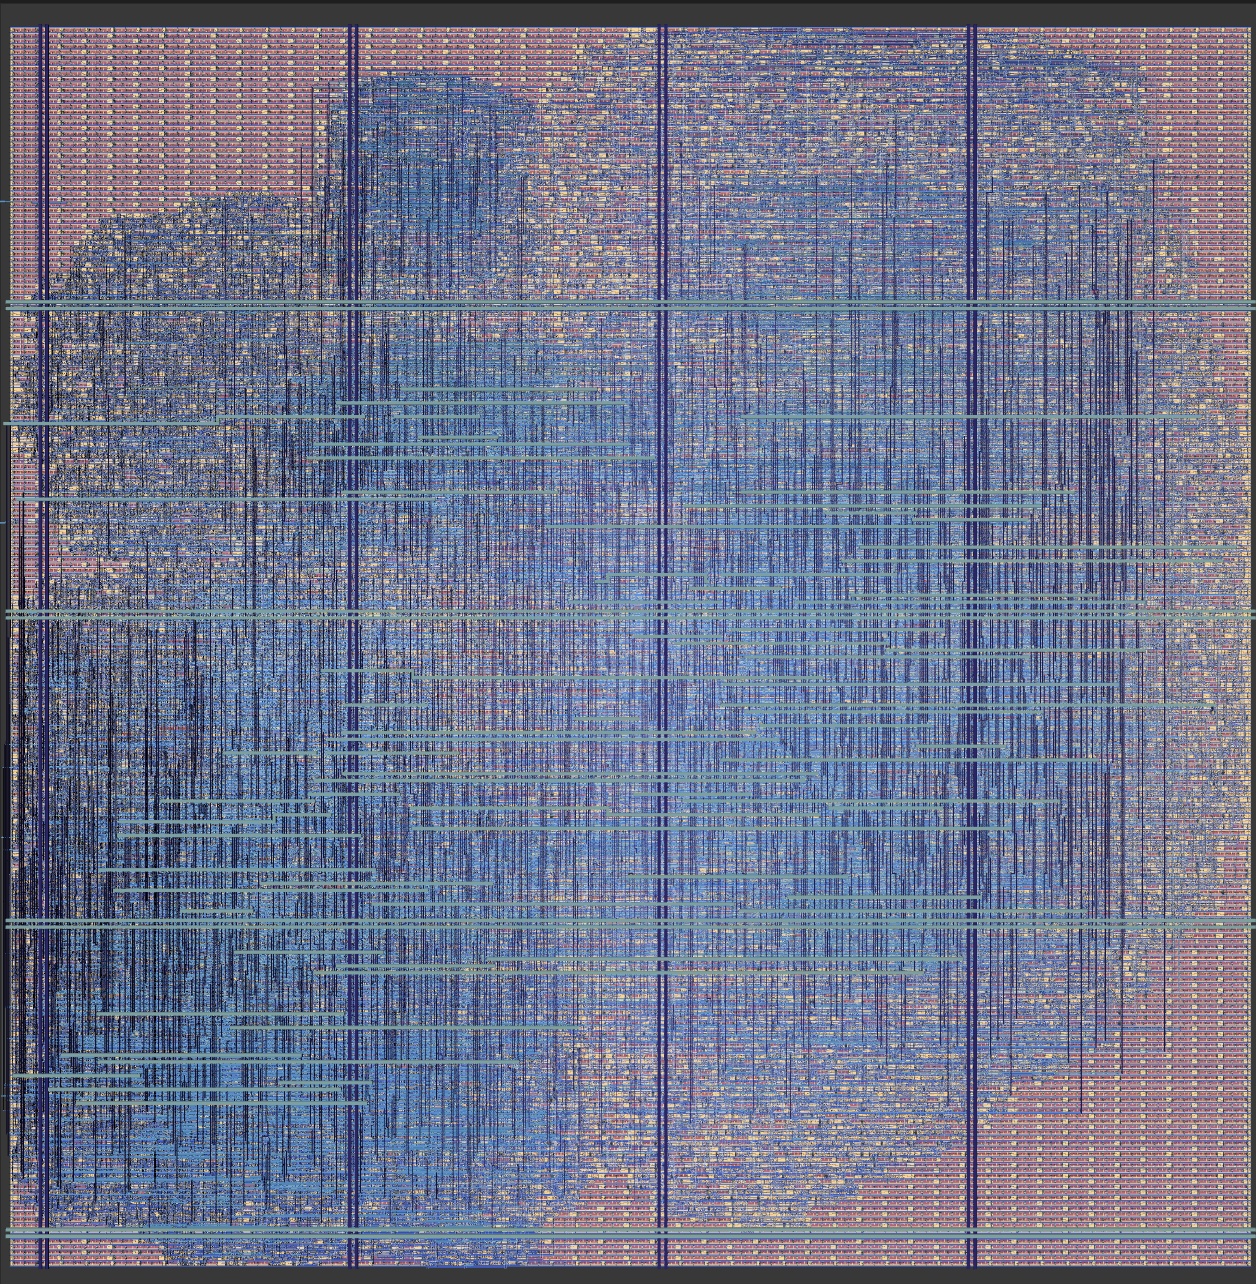
\includegraphics[width=\linewidth]{figures/gds_layout.png}\\[2pt]
  {\footnotesize\textbf{(a)} the finished layout}
\end{minipage}\hfill
\begin{minipage}[b]{0.565\linewidth}\centering
  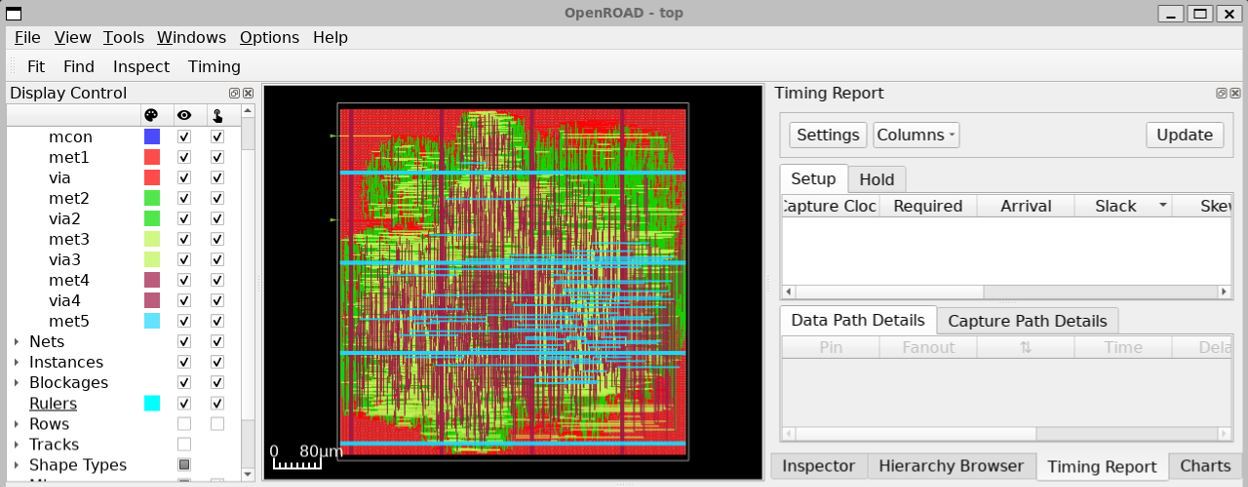
\includegraphics[width=\linewidth]{figures/openroad_heatmap.png}\\[2pt]
  {\footnotesize\textbf{(b)} the same layout, by metal layer}
\end{minipage}
\caption{The signed-off layout. \textbf{(a)} The complete die. It measures
630.15\,$\times$\,640.87\,\textmu m, or 0.404\,mm$^2$, and is 52.28\,\% full. It contains
17{,}708 standard cells. Two independent checkers found zero design-rule violations, and the
layout-versus-schematic check matched the netlist uniquely. \textbf{(b)} The same layout in
the OpenROAD viewer, with the metal layers coloured: red is \texttt{met1}, green is
\texttt{met2} and \texttt{met3}, and light blue is \texttt{met5}. The wiring is spread
evenly, with no dense spot. This agrees with the zero routing violations in
Table~\ref{tab:signoff}. The timing panel on the right lists no failing path.}
\label{fig:gds}
\end{figure}

\subsection{What was synthesised, stated precisely}

Two reductions apply to the place-and-route netlist, both on the organisers' instruction,
and both are visible in the run's own logs rather than only in our source. They are stated
here rather than buried, because a reviewer who finds them unannounced would be right to
discount everything else.

\begin{table}[htbp]
\centering\small
\caption{The two synthesis reductions, the evidence for each in the submitted run, and why
each is correct rather than convenient.}
\label{tab:reductions}
\begin{tabularx}{\linewidth}{>{\raggedright\arraybackslash}p{3.3cm}>{\raggedright\arraybackslash}p{5.4cm}X}
\toprule
\hrow \hdr{Reduction} & \hdr{Evidence in the submitted run} & \hdr{Why it is sound} \\
\midrule
\texttt{DMEM\_WORDS = 8} (32 bytes instantiated, not the full 8\,kB) &
The synthesis log records \texttt{Parameter DMEM\ub WORDS = 8}. The cell report agrees:
it counts 256 flip-flops, which is 8 words of 32 bits. &
A guard keeps every address in the 8\,kB window defined. Past the end of the array, reads
give 0 and writes do nothing. No address can alias onto a real word. Block Guide \S4.3
permits a smaller array. \textbf{The size is the smallest that works, not an arbitrary
choice:} 1, 2 and 4 words all \emph{fail} the firmware (\texttt{x4 = ffffffff}); 8
\emph{passes}. The firmware uses 28 bytes. \\
\addlinespace
3-instruction mock ROM in place of the 742-word firmware ROM &
The file the tool actually read declares the program memory with three entries instead
of 742. That file is generated from the exported netlist by a script. Nobody edits it by
hand. &
The firmware repository gives this advice itself: a 742-word \texttt{case} block ``can
generate unnecessary cells''. The mock has the same module name and the same ports, so
nothing on the canvas changes. It cannot go stale unnoticed: gate 8 builds the
\emph{whole core} against the mock and runs the repository's own three-instruction
program to \texttt{x7 = 15}. \\
\bottomrule
\end{tabularx}
\end{table}

The full 8\,kB window needs 65{,}536 flip-flops. Measured locally, that is 2.43\,mm$^2$ of
standard cells, about 95\,\% of the design, and it does not fit in this die. The functional
design on the canvas keeps all 2{,}048 words, and gate 11 checks that on the exported
netlist.

\subsection{Three results worth reading}

\begin{minipage}[t]{0.485\linewidth}
\vspace{0pt}
\textbf{1. Instance order is an area knob, worth 12\,\%.} The platform's generated
\texttt{hdl.v} and the local reproduction are identical in every module body, in the
top-level wire list, and in the resolved OpenLane environment. They differ in exactly one
thing: where the \texttt{imem} block sits in the instance list. Moving that single
instantiation, changing \emph{no logic whatsoever}, reproduces the platform's synthesis to
the byte. Yosys derives modules in instantiation order, which changes internal ID
allocation, which changes the visit order of order-sensitive passes
(\texttt{opt\_merge}, \texttt{share}, \texttt{fsm}, \texttt{opt\_muxtree}). Two consequences
carry forward: canvas block order is a free area knob, and \emph{a cell-count difference
between two runs is not by itself evidence that the RTL changed}.

\vspace{4pt}
{\scriptsize
\begin{tabularx}{\linewidth}{Xrr}
\toprule
\hrow & \hdr{\texttt{imem} 5th} & \hdr{\texttt{imem} last} \\
\midrule
Pre-ABC cells & 17{,}073 & \textbf{19{,}080} \\
\texttt{\$\_XNOR\_} / \texttt{\$\_XOR\_} & 941 / 2{,}644 & \textbf{1{,}386 / 3{,}064} \\
Mapped cells & 15{,}524 & \textbf{17{,}708} \\
Cell area (\textmu m$^2$) & 171{,}332 & \textbf{191{,}649} \\
\bottomrule
\end{tabularx}}
\end{minipage}\hfill
\begin{minipage}[t]{0.485\linewidth}
\vspace{0pt}
\textbf{2. Heuristic antenna-diode insertion cost 19.5\,\% of the die for nothing.}
\texttt{RUN\_HEURISTIC\_DIODE\_INSERTION} places a diode pre-emptively on nearly every net.
It inserted \textbf{9{,}838} diodes, a 63\,\% cell-count increase applied \emph{after} the
floorplan had already been sized, and left \emph{exactly the same} residual violating nets
at signoff as targeted repair with \textbf{325}. Disabling it shrank the die from
666\,$\times$\,676 to 596\,$\times$\,607\,\textmu m ($-$19.5\,\%), returned $\approx$1.9\,ns
of setup slack, and turned a \texttt{GRT-0119} routing-congestion failure into a clean route.
This is why \texttt{config.json} sets it to \texttt{0} explicitly.

\vspace{3pt}
\textbf{3. Reported frequency versus achieved margin, both stated honestly.} The run reports
\textbf{30.303 MHz}, but that figure only ever echoes the constraint: OpenLane clamps
positive slack to zero (\texttt{wns = 0.0}) before computing
\texttt{suggested\_clock\_frequency}. The design actually closes with 2.25\,ns to spare at
the slow corner, i.e.\ at $\approx$30.75\,ns, or \textbf{$\approx$32.5 MHz} on this run.
Two caveats we state rather than omit: slack varied by 1.6\,ns run-to-run on identical
inputs, and the local run series measured a required period of 32.36\,ns regardless of the
target. \textbf{Treat 33\,ns as the guaranteed constraint and $\approx$32.5 MHz as a
single-run demonstration, not a characterised $f_\text{max}$.}
\end{minipage}

\subsection{Residual issues, reported rather than papered over}

\begin{itemize}
\item \textbf{Residual antenna violations: 86 pins on 60 nets}, worst partial/required ratio
  \textbf{8.69$\times$} the 400 limit, mostly on met3. Enabling heuristic diode insertion
  does \emph{not} reduce them, and costs 19.5\,\% of the die, so they are recorded rather
  than papered over. They do not affect DRC, LVS or the routing result.
\item \textbf{Max-slew and max-fanout warnings at the typical corner.} The default
  \texttt{MAX\ub FANOUT\ub CONSTRAINT} is 10; the offenders are high-fanout control and
  operand-broadcast nets. Real signoff warnings, but not what limits $f_\text{max}$.
\item \textbf{IR-drop analysis is approximate} (\texttt{VSRC\_LOC\_FILES} unset), which is
  expected for a design that is not a top-level chip integration.
\item \textbf{No timing-annotated simulation was run after layout.} We did compare the
  design against the \emph{post-synthesis} netlist for 900 cycles, and the results were
  identical. Signoff timing analysis also reports positive margin at every corner. However,
  we did not keep the 88\,MB timing file, and we did not run a gate-level simulation with it.
  This is the one gap in the flow, and we state it as such.
\end{itemize}


% =============================================================================
% 6 FIRMWARE DEMO
% =============================================================================
\section{Firmware Demo}
\label{sec:firmware}

\textbf{In one paragraph.} The official ChampionCHIP validation firmware runs on this core.
It returns \textbf{\texttt{x4 = 0x00000000}}, which is its own PASS value. It reaches that
result after \textbf{991 clock cycles} and then stops in its \texttt{all\_good} loop. The
firmware contains nine test stages, one after the other. \textbf{All nine complete.}

The firmware does not use \texttt{ECALL} or \texttt{EBREAK} to report that it has finished.
It ends with \texttt{j .}, an instruction that jumps to itself. The testbench therefore
watches the program counter. When the program counter stops at one of the two exit loops,
the firmware has finished, and the testbench reads the result from register \texttt{x4}.

Every stage that fails jumps to the same error label. A single failure would therefore hide
which stage caused it. To prevent this, the testbench records the address the jump came
from. That address identifies the stage.

\begin{table}[htbp]
\centering\scriptsize
\caption{All nine validation stages of the official firmware, and the evidence each
completed. PC ranges are the branch-source attribution boundaries the testbench uses to name
a failing stage. Because the stages are sequential and each ends in a conditional branch to
\texttt{\_error}, reaching \texttt{all\_good} at \texttt{0x004003E8} is proof that
\emph{every} stage passed. There is no path to it that skips one. The stage names and
their address ranges are taken from the competition firmware's own source listing.}
\label{tab:stages}
\setlength{\tabcolsep}{4pt}
\begin{tabularx}{\linewidth}{c>{\ttfamily\scriptsize}p{2.85cm}>{\ttfamily\scriptsize}p{2.75cm}Xc}
\toprule
\hrow \hdr{\#} & \normalfont\bfseries Stage & \normalfont\bfseries PC range &
\hdr{What it exercises} & \hdr{Result} \\
\midrule
1 & \_rv32i\_alu\_test & 00400000--00400118 &
  \texttt{LUI}, \texttt{AUIPC}, \texttt{ADDI}/\texttt{ADD}/\texttt{SUB}, all logic ops,
  \texttt{SLL}/\texttt{SRL}/\texttt{SRA} including \texttt{SRAI} with a shift amount
  requiring \texttt{b[4:0]} masking, \texttt{SLT}/\texttt{SLTU} at the signed/unsigned
  boundary & \ok \\
2 & \_rv32i\_lsu\_test & 0040011C--00400180 &
  \texttt{.bss} base derived from the PC (\texttt{auipc s0,0xfc10} $\to$
  \texttt{0x10010000}); \texttt{SW}/\texttt{SH}/\texttt{SB} then
  \texttt{LW}/\texttt{LH}/\texttt{LHU}/\texttt{LB}/\texttt{LBU}: all eight width/offset
  combinations & \ok \\
3 & \_rv32i\_ctrl\_test & 00400184--0040020C &
  All six branch conditions in both directions, including negative operands
  (\texttt{-10}) that separate signed from unsigned comparison; \texttt{JAL} and
  \texttt{JALR} control transfer & \ok \\
4 & \_rv32i\_reg\_test & 00400210--00400234 &
  Register-file integrity: \texttt{addi zero, zero, 1} followed by
  \texttt{bne zero, zero, \_error} probes the \texttt{x0} hardwiring; a value is propagated
  through \texttt{x5}$\to$\texttt{x6}$\to$\texttt{x7}$\to$\texttt{x31} & \ok \\
5 & \_rvbl2\_mult\_test & 00400238--00400294 &
  All four Zmmul instructions with operands chosen to separate them:
  $100000\times2$, an $8\times10^9$ product exercising the upper half, and a
  \texttt{MULHSU} case that distinguishes signed$\times$unsigned from both alternatives & \ok \\
6 & \_rvbl2\_crc\_test & 00400298--00400348 &
  \texttt{CRCB}/\texttt{CRCH}/\texttt{CRCW} chained to the firmware's own expected
  \texttt{0x1E82}. \textbf{This stage found a real bug:} the CRC block took its two
  operands the wrong way round. Earlier tests could not see it, because
  \texttt{CRCH} gives the same answer either way & \ok \\
7 & \ub rvbl2\ub crc\ub mem\ub test & 0040034C--00400374 &
  \texttt{LW} of \texttt{.rodata} located \emph{in the instruction ROM} at
  \texttt{0x004003F8}, then \texttt{CRCW} over it: the exact case the datapath's
  extended \texttt{oe\_o}/address scoping exists for & \ok \\
8 & \ub rvbl2\ub arith\ub integ\ub test & 00400378--00400390 &
  Integration: $(A+B)\times(A-B)$ across \texttt{ADD}, \texttt{SUB} and \texttt{MUL} in
  sequence, checking that results feed correctly between instruction classes & \ok \\
9 & \ub rvbl2\ub mem\ub transfer\ub test & 00400394--004003E4 &
  A three-word copy loop reading its source from the ROM at \texttt{0x00400400} and writing
  to data memory, then reading the destination back: loads, stores, pointer arithmetic
  and a backward branch together & \ok \\
\midrule
\hrow \multicolumn{4}{l}{\normalfont\textbf{Verdict: \texttt{all\_good} at
  \texttt{0x004003E8}: \texttt{li x4, 0} ; \texttt{j .}}} &
  \normalfont\textcolor{okgreen}{\textbf{9/9}} \\
\bottomrule
\end{tabularx}
\end{table}

\vspace{-4pt}
\subsection{Testbench log output proving the run reached the end without errors}

\begin{lstlisting}[caption={The platform testbench's own output, verbatim. \texttt{SUITE 2A}
is the official validation firmware; the surrounding suites are the project's own coverage.
\texttt{SUITE 3} re-runs the official firmware after injecting reset at 40 different points
of its execution and confirms it still returns \texttt{x4=00000000}.},
label={lst:fwlog},captionpos=b]
============================================================
 RVBL-2 combined verification suite
 RV32I + Zmmul + Xicrc, 47 instructions
============================================================
-- SUITE 0: unit tests (core held in reset) -----------------
  CHECK-VALUE GATE: chained CRCB("123456789") = 0x29b1 (expected 0x29B1) PASS
  [S0.8] CRC-16/CCITT-FALSE: KAT gate, firmware 0x1E82 anchor, corners, 600 randomised
-- SUITE 1: control unit ------------------------------------
  [S1.1] Control decode sweep: 704 encodings through the real FSM
-- SUITE 2A: OFFICIAL VALIDATION FIRMWARE --------------------
  Firmware settled after 991 cycles at pc=004003ec (all_good)
  ******************************************************
  *  OFFICIAL VALIDATION FIRMWARE: x4 = 00000000  PASS  *
  ******************************************************
  [S2A] Official validation firmware: 991 cycles, verdict x4=00000000
-- SUITE 2B: integration, supplementary coverage program -----
  [sys_event_o pulse #1] cycle=1854 pc=00400f50
  [sys_event_o pulse #2] cycle=1950 pc=00400f88
  Ran 6000 cycles, observed 2 sys_event_o pulses (expect 2: EBREAK then ECALL)
  Signature-based instruction tests: 58/58 passed
-- SUITE 3: reset stress ------------------------------------
  [S3.1] Reset injected at 40 points of the official firmware: writes aborted, PC/FSM/GPRs cleared
  [S3.2] Reset recovery: the official firmware still returns x4=00000000 after 991 cycles
============================================================
==== testbench: 15281 passed, 0 failed ====
ALL TESTS PASSED
============================================================
\end{lstlisting}

\begin{lstlisting}[caption={The reference regression, run block by block against the
reference design, and copied into this report without editing. \texttt{tb\_gatelevel} needs
a synthesised netlist. When that netlist is absent the suite skips this testbench and does
not fail it. With it, the suite is 16 of 16 and 8{,}285 checks.},
label={lst:runall},captionpos=b]
==============================================
 Unit-level testbenches
==============================================
PASS          tb_alu                   ==== tb_alu: 1128 passed, 0 failed ====
PASS          tb_branch_comparator     ==== tb_branch_comparator: 24 passed, 0 failed ====
PASS          tb_immediate_generator   ==== tb_immediate_generator: 34 passed, 0 failed ====
PASS          tb_register_file         ==== tb_register_file: 36 passed, 0 failed ====
PASS          tb_multiplier            ==== tb_multiplier functional: 2198 passed, 0 failed ====
PASS          tb_crc_unit              ==== tb_crc_unit: 322 passed, 0 failed ====
PASS          tb_lsu                   ==== tb_lsu: 26 passed, 0 failed ====
PASS          tb_imem                  ==== tb_imem: 7 passed, 0 failed ====
PASS          tb_dmem                  ==== tb_dmem: 17 passed, 0 failed ====
PASS          tb_address_decoder       ==== tb_address_decoder: 12 passed, 0 failed ====
PASS          tb_control_unit          ==== tb_control_unit: 1461 passed, 0 failed ====
==============================================
 Integration-level testbenches
==============================================
PASS          tb_core      ==== tb_core: 29 passed, 0 failed ====
PASS          tb_soc       ==== tb_soc: 14 passed, 0 failed ====
PASS          tb_reset     ==== tb_reset: 2002 passed, 0 failed (40 injection points) ====
PASS          tb_firmware  ==== tb_firmware: 70 passed, 0 failed ====
              TB_FIRMWARE: ALL TESTS PASSED (47/47 instructions verified)
==============================================
 SUMMARY: 15/15 testbenches passed, 7384 individual checks
==============================================
\end{lstlisting}

\subsection{Waveform evidence}

A waveform is a picture of the simulation. Time runs from left to right. Each row is one
signal. A single-bit signal is drawn as a square wave, high or low. A multi-bit signal is
drawn as a stretched hexagon with its value written inside, and the hexagon pinches at each
point where the value changes. The clock row gives the scale: one full high-low pair is one
clock cycle, which is 10\,ns here.

The two figures below come from one simulation run. That run executes the competition test
program on the netlist the platform exported.

\figorbox{figures/wave_firmware.png}{0.99\linewidth}
  {Validation firmware waveform.}
  {The competition test program completing. Panel A is a summary of the whole run. Each
   numbered band is one of the nine test stages, drawn to scale in time, and the red band at
   the right is the result. Panel B magnifies the last 100\,ns. The core executes
   \texttt{addi x4, x0, 0}, which writes the PASS value into the verdict register: the
   \texttt{rd\_addr} row shows \texttt{x4}, the \texttt{rd\_data} row shows
   \texttt{00000000}, and \texttt{reg\_write} goes high for one cycle in \textsc{wb}. The
   red line marks that write taking effect. The core then executes \texttt{j .}, a jump to
   itself, so the \texttt{pc} row stops at \texttt{004003ec} and never moves again.}
  {fig:wavefw}

\begin{callout}{What Figure~\ref{fig:wavefw} proves}
The program only reaches \texttt{addi x4, x0, 0} if every one of the nine stages passed.
Each stage ends with a branch to a shared error label, and that label writes $-1$ instead.
The waveform shows the PASS write happening and the program counter stopping, so no stage
branched away. Panel A shows the nine stages in sequence, which is the evidence
Submission Guide \S6 asks for.
\end{callout}

\figorbox{figures/wave_instruction.png}{0.99\linewidth}
  {Instruction-level waveform.}
  {One \texttt{CRCB} instruction of the custom Xicrc extension, executing in four clock
   cycles. The \texttt{state} row steps
   \textsc{fetch}\,$\to$\,\textsc{decode}\,$\to$\,\textsc{execute}\,$\to$\,\textsc{writeback},
   which matches the four-cycle path in Figure~\ref{fig:fsm}. The operands are visible:
   \texttt{crc.rs1\_data} carries the data byte \texttt{0x12} and \texttt{crc.rs2\_data}
   carries the running checksum \texttt{0xFFFF}. The answer \texttt{0xD383} appears on
   \texttt{crc.result} during \textsc{decode} and stays steady, because the CRC block is
   combinational and has no clock. \texttt{wb\_src\_sel} reads \texttt{2 crc}, so the
   writeback multiplexer selects the CRC port. The green line is the
   \textsc{writeback}\,$\to$\,\textsc{fetch} edge, where register \texttt{x8} captures the
   answer.}
  {fig:waveinst}

Three things in Figure~\ref{fig:waveinst} are worth reading carefully, because together they
show the whole datapath working on one instruction.

\begin{enumerate}[leftmargin=1.35em,itemsep=1pt,topsep=2pt]
\item \textbf{The result is ready before it is needed.} \texttt{crc.result} settles during
  \textsc{decode}, one full cycle before \textsc{writeback} uses it. This is expected: the
  CRC block is pure logic, so its output follows its inputs with no clock. \textsc{execute}
  therefore spends its cycle on a value that is already correct. The same is true of the ALU
  and the multiplier, which is why this processor needs no result register between states.
\item \textbf{The right unit is selected.} Four units compute an answer at the same time from
  the same two operands. \texttt{wb\_src\_sel} chooses which answer reaches the register
  file. It reads \texttt{2 crc} here, and it would read \texttt{0 alu} for an addition.
\item \textbf{The answer is chained.} Immediately after the green edge,
  \texttt{crc.rs2\_data} changes from \texttt{0000ffff} to \texttt{0000d383}. The next
  \texttt{CRCB} has read back the value this one just wrote. A checksum is built one byte at
  a time, so this hand-off is the instruction doing its job.
\end{enumerate}

An independent check confirms the number. The standard CRC-16/CCITT-FALSE algorithm, applied
to the byte \texttt{0x12} with the start value \texttt{0xFFFF}, gives \texttt{0xD383}. That
is the value on \texttt{crc.result}.

\subsection{Verification beyond the verdict register}

The verdict register alone is not sufficient proof. The firmware checks its own work with
branches, and those branches read the same registers the firmware has just written. A core
could therefore calculate every comparison correctly, write the results to the wrong
addresses, and still leave \texttt{x4 = 0}.

The testbench closes this gap. It examines the data memory \emph{directly}, without using
any branch the firmware used. It checks six words against values calculated outside the
design: words 0, 1 and 2, which stage 2 wrote with a store-word, a store-half and a
store-byte; and words 4, 5 and 6, which the copy loop of stage 9 wrote. It also confirms
that register \texttt{x0} is still zero after the complete run.

Words 4 to 6 prove one more thing. The copy loop reads its source data from
\texttt{0x00400400}, which is an address in the program memory. Correct values in those
words therefore show that a load from the program memory works from end to end.



% =============================================================================
% CLOSE
% =============================================================================
\section{Video, Deliverables and Reproduction}
\label{sec:deliverables}

\begin{center}
\setlength{\fboxsep}{8pt}%
\fcolorbox{rvbl}{rvblsoft}{\begin{minipage}{0.94\linewidth}\centering
{\color{rvbl}\bfseries\large Project demonstration video (Submission Guide \S7)}\\[4pt]
\large\url{\videourl}\\[3pt]
{\footnotesize Covering project architecture, processor operation, system simulation,
firmware execution, OpenLane results and the final chip layout.}\\[7pt]
{\color{rvbl}\bfseries\large Public repository}\\[4pt]
\large\url{\repourl}\\[3pt]
{\footnotesize The complete design, both testbench suites, the equivalence proof and every
figure in this report at full resolution.}
\end{minipage}}
\end{center}

\begin{minipage}[t]{0.55\linewidth}
\vspace{0pt}\footnotesize
\captionof{table}{Submission Guide \S9 expected files, and where each is in the submission.}
\label{tab:deliverables}
\begin{tabularx}{\linewidth}{>{\raggedright\arraybackslash}p{2.5cm}X}
\toprule
\hrow \hdr{Required} & \hdr{Location} \\
\midrule
Report & This document \\
GDSII layout & The complete OpenLane run directory, under its
  \texttt{results} folder \\
Gate-level netlist & The same run directory. Both the powered and the
  non-powered netlist are included \\
Synthesis configuration & The twelve-key \texttt{config.json} that was submitted,
  together with the platform's own record of what it received \\
All code and testbenches & 16 reference design files, 16 reference testbenches, and the
  ChipInventor set: 18 block sources, the platform testbench, the firmware and the
  build scripts \\
Video link & Above, and on the title page \\
\bottomrule
\end{tabularx}
\end{minipage}\hfill
\begin{minipage}[t]{0.42\linewidth}
\vspace{0pt}
\subsection*{\color{rvbldark}Reproducing every claim}
\small
Both suites are self-checking and exit non-zero on any failure. Icarus Verilog and Python 3
are the only requirements.

\vspace{3pt}
Run \texttt{run\ub all.sh} for the reference regression: 15 testbenches and 7{,}384 checks.
Run \texttt{run\ub ci.sh} for the ChipInventor chain: 12 gates, 15{,}281 checks, and the
competition firmware verdict. Both scripts print a pass or fail line for every gate and
return a non-zero exit code if any gate fails.

\vspace{3pt}
To repeat the physical run, enter the twelve configuration keys into the ChipInventor
synthesis page. The same result can be produced locally with the pinned toolchain: OpenLane
build \texttt{3876562d} with the sky130A process kit \texttt{bdc9412b}. Two setup scripts in
the submission do this.
\end{minipage}

\subsection*{\color{rvbl}Conclusion}

RVBL-2 implements all 47 instructions that the competition specifies. It uses the
multicycle arrangement that the Block Guide requires, and it was built on the ChipInventor
platform. The result is a signed-off Sky130A layout of 0.404\,mm$^2$ at 52.28\,\% density,
with zero design-rule violations, a unique LVS match, and 2.25\,ns of setup margin at the
slow corner. The organisers' own validation firmware completes all nine of its stages and
returns its PASS verdict.

The most important property is not any single number. It is the chain that connects them
(Figure~\ref{fig:chain}). The netlist that OpenLane built is provably the same netlist that
the testbenches verified. Two checks prove this: a cycle-by-cycle comparison over 410{,}400
points, and a structural comparison of the platform's own export that does not depend on
instance names. Neither is an assertion.

The design has four real limits. This report states each one with its measurement.
\begin{enumerate}[leftmargin=1.35em,itemsep=1pt,topsep=2pt]
\item The place-and-route netlist contains 8 data words, not 2{,}048. The organisers
  instructed this reduction. Simulation shows that 8 words is the smallest size that still
  passes validation.
\item 86 antenna pins remain. The standard remedy was measured. It costs 19.5\,\% of the die
  area and removes none of them.
\item The tool reports 30.3\,MHz. That figure repeats the constraint we set. The frequency
  the run actually demonstrates is about 32.5\,MHz, and repeated runs vary by 1.6\,ns.
\item No timing-annotated simulation was run after layout.
\end{enumerate}

\needlines{12}
\subsection*{\color{rvbldark}Result against each Submission Guide topic}

\vspace{-2pt}
{\small
\begin{tabularx}{\linewidth}{c>{\raggedright\arraybackslash}p{3.3cm}X}
\toprule
\hrow \hdr{\S} & \hdr{Topic} & \hdr{Measured result} \\
\midrule
1 & Project Overview & 47 instructions in a 6-state multicycle core; 17 block
    definitions placed as 20 instances; 3 to 5 cycles per instruction \\
2 & Supported Instructions & 47 of 47 implemented, all ten categories at
    100\,\%, each with a directed test that passes \\
3 & Datapath & One ALU, one memory port and five multiplexers, shared over time
    by the state machine; every net in Figure~\ref{fig:datapath} is real \\
4 & Modules and Testbenches & 15{,}281 checks in the platform suite and 8{,}285
    in the reference suite, 0 failures; 12 automatic gates all pass \\
5 & OpenLane Results & 0.404\,mm$^2$ at 52.28\,\% density; 0 DRC from two
    independent checkers; LVS matches uniquely; $+2.25$\,ns setup margin at the
    slow corner \\
6 & Firmware Demo & All nine validation stages complete and the firmware returns
    \texttt{x4 = 0x00000000} after 991 cycles \\
\bottomrule
\end{tabularx}}

\vspace{6pt}
\subsection*{\color{rvbldark}Why the two test suites are independent}

The reference suite and the platform suite were written against the same
specification but not against each other. The reference suite tests sixteen separate design
files with expected values calculated in Python. The platform suite tests the single
combined file that ChipInventor actually runs, with expected values calculated by reference
functions inside the testbench. The two use different sources for their expected values, so
a fault would have to appear in both, in the same way, to pass unnoticed.

A third check is stronger still, because it needs no expected values at all. The mirror
equivalence test runs the canvas design and the reference design side by side for 410{,}400
cycles and compares the complete architectural state at every cycle. It reports zero
mismatches. Whatever the two designs do, they do the same thing.

\end{document}
